\documentclass[article, onecolumn]{IEEEtran}

\usepackage{cite}
\ifCLASSINFOpdf
	\usepackage[pdftex]{graphicx}
	\graphicspath{{./tikz_figures/}}
	\DeclareGraphicsExtensions{.pdf,.jpeg,.png, .jpg, .PNG}
\else
\fi
\usepackage{amsmath,bm}
\interdisplaylinepenalty=2500
\ifCLASSOPTIONcompsoc
	\usepackage[caption=false,font=normalsize,labelfont=sf,textfont=sf]{subfig}
\else
	\usepackage[caption=false,font=footnotesize]{subfig}
\fi
\usepackage{url}
\usepackage{amsfonts} % for \mathbb{}
\usepackage{listings} % For writing math in verbatim
\usepackage{enumerate}

\usepackage[showlabels,sections,floats,textmath,displaymath]{preview}
\usepackage{amssymb} %% For showing special symbols like \bigstar
\usepackage{pifont}  %% For showing circled numbers
\usepackage{array}
\usepackage{algorithm}
\usepackage{algpseudocode}
\usepackage{ifthen}
\usepackage{dirtree}
\setlength{\DTbaselineskip}{13pt}
\renewcommand*\DTstyle{}
\DTsetlength{.2em}{1em}{.2em}{.4pt}{2pt}

\newcommand{\mathnew}{\mathit} 
% for nice reference 
\newcommand{\fsp}{{\;}}
\newcommand{\Fig}{\figurename \fsp}
\newcommand{\Sec}{Sec.\fsp}
\newcommand{\Eq}{Eq.\fsp}
\newcommand{\Tab}{Tab.\fsp}
\newcommand{\Alg}{Alg.\fsp}
\newcommand{\etal}{\textit{et al}. }
\newcommand{\ie}{\textit{i}.\textit{e}. }
\newcommand{\eg}{\textit{e}.\textit{g}. }
\newcommand{\Prop}{Property }

\DeclareMathOperator*{\argminB}{argmin} 

\hyphenation{temperature} % correct bad hyphenation here

\usepackage{tikz}
\usetikzlibrary{arrows}
\usetikzlibrary{intersections}
\usetikzlibrary{calc, quotes}
\usetikzlibrary{external}
\tikzexternalize[prefix=tikz_figures/]%
\pgfdeclarelayer{bg}    % declare background layer
\pgfsetlayers{bg,main} % set the order of the layers (main is the standard layer)
\usetikzlibrary{patterns, patterns.meta}
\usetikzlibrary{decorations.pathreplacing,calligraphy}

\renewcommand\thesection{\arabic{section}}
\renewcommand\thesubsectiondis{\textbf{\thesection.\arabic{subsection}}} %% This is to change the looking of subsection heading number
\renewcommand\thesubsection{\thesection.\arabic{subsection}} %% This is to change the numbering by \ref{}
\renewcommand\thesubsubsectiondis{\ding{42}\;\thesection.\arabic{subsection}.\arabic{subsubsection}}

\setcounter{tocdepth}{1} % Show sections
%\setcounter{tocdepth}{2} % + subsections
%\setcounter{tocdepth}{3} % + subsubsections
%\setcounter{tocdepth}{4} % + paragraphs
%\setcounter{tocdepth}{5} % + subparagraphs

%% The following commands are used to reduce the space before and after formula
%% in align and equation environments
%\setlength{\abovedisplayskip}{1pt}
%\setlength{\belowdisplayskip}{0pt}
%\setlength{\abovedisplayshortskip}{0pt}
%\setlength{\belowdisplayshortskip}{0pt}

%%
%% The following definition is a remedy of the fact that
%% IEEEtrans class does not define subparagraph.
%% Check this post for details
%% https://tex.stackexchange.com/a/8362/172530
\newcommand{\subparagraph}{}
\usepackage{titlesec} % for controlling vertical space around section headers
\titlespacing\section{0pt}{8pt plus 2pt minus 2pt}{4pt plus 2pt minus 2pt}
\titlespacing\subsection{0pt}{6pt plus 2pt minus 2pt}{2pt plus 2pt minus 2pt}
\titlespacing\subsubsection{0pt}{4pt plus 2pt minus 2pt}{2pt plus 1pt minus 1pt}

\titleformat{\subsection}
{\normalfont\bfseries}
{\thesubsection}{1em}{}

%%
%% Check this post for how to write properly-sized ceiling operator
%% https://tex.stackexchange.com/a/367035/172530
%%
\usepackage{mathtools}
\DeclarePairedDelimiter{\ceil}{\lceil}{\rceil}
\DeclarePairedDelimiter{\floor}{\lfloor}{\rfloor}

%% For text color
\usepackage{xcolor}

%% For drawing boxes around text
%% https://tex.stackexchange.com/a/234195/172530
\newcommand\textbox[2]{%
  \tikz[baseline]\node[%
  inner ysep=0pt, 
  inner xsep=2pt, 
  anchor=text, 
  rectangle, 
  rounded corners=1mm,
  #1] {\strut#2};%
}

%% package for highlighting text
%% Usage: \hl{text to be highlighted}
\usepackage{soul}
\sethlcolor{yellow}

%% underlining for emphasis
%% Examples:
%% \uline{important} underline
%% \uuline{urgent} double-underline
%% \uwave{boat} wavy underline like
%% \sout{wrong} line struck through word
%% \xout{removed} removed
%% \dashuline{dashing} dashed
%% \dotuline{dotty} dotted
\usepackage[normalem]{ulem}

%% define a red check mark
\newcommand\redcheck{
  {\textcolor{red}{\ding{52}}}
}

\usepackage{dblfloatfix}    % To enable figures at the bottom of page

\usepackage{wrapfig}
\usepackage{siunitx}

% Overlay question mark on equal mark
\def\qeq{\mathrel{%
    \mathchoice{\QEQ}{\QEQ}{\scriptsize\QEQ}{\tiny\QEQ}%
}}
\def\QEQ{{%
    \setbox0\hbox{=}%
    \rlap{\hbox to \wd0{\hss?\hss}}\box0
  }}

%% Package for theorem-like blocks
\usepackage{amsthm}
\renewcommand\qedsymbol{$\blacksquare$}
\newtheorem{prop}{Property}

%%%%%%%%%%%%%%%%%%%%%%%%%%%%%%%%%%%%%%%%%%%%%%%%%%%%%%%%%%
%% Tikz figure commands
%%%%%%%%%%%%%%%%%%%%%%%%%%%%%%%%%%%%%%%%%%%%%%%%%%%%%%%%%%
\newcommand{\defs}[1]{
  %% #1: gap
  \def\latalu{6}
  \def\latmem{24}
  \def\unit{.1}
  \def\h{.2}
  \def\scale{.7}
  \def\alpha{6}
  \def\numwarps{6}
  \def\gap{#1}
  \pgfmathsetmacro\latwarp{\alpha*\latalu*\unit+\latmem*\unit+\alpha*\gap*\unit-\gap*\unit}
  \pgfmathsetmacro\span{\alpha*\latalu+\latmem+\alpha*\gap-\gap+\numwarps-1}
}

\newcommand{\cycles}[2]{
  %% #1: height of the line
  %% #2: number of cycles
  \foreach \i in {0,...,#2}
  {
    \draw [ultra thin, red] ($(TL)+(\i*.1, 0)$) -- ++(0, -#1);
  }
}

\newcommand{\mylabel}[4]{
  %% #1 width of the label
  %% #2 text for the label
  %% #3 scale
  %% #4 below of above
  %% The left is defined as the coordinate before calling this command
  \coordinate (right) at ($(left)+(#1, 0)$);
  \node [scale=#3, #4, inner xsep=0] (label) at ($(left)!.5!(right)$) {#2};
  \draw [ultra thin] (left) |- (label.west); 
  \draw [ultra thin] (right) |- (label.east); 
}

\newcommand{\latlabel}[1]{
  %% #1: scale of the text
  %% (left) should be defined as the topleft of the warp
  \mylabel{\latalu*\unit}{$\text{lat}_\text{alu}$}{\scale}{above};
  \coordinate (left) at ($(left)+(\alpha*\latalu*\unit+\alpha*\gap*\unit-\gap*\unit, 0)$);
  \mylabel{\latmem*\unit}{$\text{lat}_\text{mem}$}{\scale}{above};
}

\newcommand{\coord}[3]{
  %% origin is defined as a coordinate
  %% #1: x length
  %% #2: y length
  %% #3: scale
  \draw [fill=black] (origin) circle (2pt);
  \draw [thick, ->, >=stealth, name path=x] (origin) -- ++(#1, 0)
  node [scale=#3, right] {$n$};
  \draw [thick, ->, >=stealth, name path=y] (origin) -- ++(0, #2)
  node [scale=#3, above] {$\text{thr}_\text{warp}$};  
}
\newcommand{\maxthralu}[4]{
  %% #1: \alpha, i.e. number of alu insts per warp
  %% #2: number of warps 
  %% #3: starting index of the first warp in this group
  %% #4: gap between consecutive alu insts
  %% (TL) should already be defined
  \pgfmathsetmacro\alp{int(#1-1)}
  \pgfmathsetmacro\warps{int(#2-1)}
  \foreach \w in {0,...,\warps} {
    \pgfmathsetmacro\z{int(#3+\w)}
    \node [left, scale=.9*\scale] at ($(TL)+(\w*\unit,-\w*\h-.5*\h)$) {w\z};
    \foreach \i in {0,...,\alp} {
      \draw [thick] ($(TL)+(\i*#4*\unit+\i*\latalu*\unit+\w*\unit, -\w*\h)$)
      rectangle ++(\latalu*\unit, -\h);
    }
  }
}

\newcommand{\maxthrmem}[1]{
  %% #1: number of warps 
  %% (memTL) should already be defined
  \pgfmathsetmacro\warps{int(#1-1)}
  \foreach \w in {0,...,\warps} {
    \draw [thick, blue] ($(memTL)+(\w*\unit, -\w*\h)$)
    rectangle ++(\latmem*\unit, -\h);
  }
}

\newcommand{\drawwarp}[4]{
  %% parameters same as \maxthralu
  %% #1: \alpha, i.e. number of alu insts per warp
  %% #2: number of warps 
  %% #3: starting index of the first warp in this group
  %% #4: gap between consecutive alu insts
  %% (TL) should already be defined
  \maxthralu{#1}{#2}{#3}{#4};
  \coordinate (memTL) at ($(TL)+(#1*\latalu*\unit+#1*#4*\unit-#4*\unit, 0)$);
  \maxthrmem{#2};
}

\newcommand{\myPerfModel}[1]{
  %% #1 scale
  
  % \draw [help lines] (-4,3) grid (4, -3);
  % \draw (0,0) circle (2pt);

  \def\scale{#1}

  %% Draw latency mode
  \coordinate (origin) at (-3,0);
  \coord{5}{3}{\scale};
  \coordinate (P) at ($(origin)+(1.5,1.5)$);
  \draw [ultra thick] (origin)
  --node [midway, above, sloped, align=center, scale=.8*\scale] {latency mode} (P);
  \draw [ultra thin, densely dashed] (P) -- (P |- origin)
  node [below, scale=\scale] {$n_\text{lat}$};
  \draw [ultra thin, densely dashed] (P) -- (P -| origin)
  node [left, scale=\scale] {$\text{thr}_\text{lat}$};
  %% Draw gradual saturate effect
  \coordinate (Q) at ($(P)+(1,.5)$);
  \draw [ultra thick] (P) to[out=40, in=185]
  node [scale=.7*\scale, midway, align=center, below, yshift=-1ex, xshift=1.5ex]
  {gradual\\saturate\\effect} (Q);
  \draw [ultra thin, densely dashed] (Q) -- (Q |- origin)
  node [below, scale=\scale] {$n_\text{thr}$};
  \draw [ultra thin, densely dashed] (Q) -- (Q -| origin)
  node [left, scale=\scale] {$\text{maxThr}_\text{warp}$};
  %% Draw throughput mode
  \draw [ultra thick] (Q) --node [midway, above, sloped, align=center, scale=.8*\scale]
  {Throughput mode} ++(2, 0);
}

\newcommand{\volkovPerfModel}[1]{
  %% #1 scale
  
  % \draw [help lines] (-4,3) grid (4, -3);
  % \draw (0,0) circle (2pt);

  \def\scale{#1}

  %% Draw latency mode
  \coordinate (origin) at (-3,0);
  \coord{5}{3}{\scale};
  \coordinate (P) at ($(origin)+(2,2)$);
  \draw [ultra thick] (origin)
  --node [midway, above, sloped, align=center, scale=.9*\scale] {latency mode} (P);
  \draw [ultra thin, densely dashed] (P) -- (P |- origin)
  node [below, scale=\scale] {$n_\text{tran}$};
  \draw [ultra thin, densely dashed] (P) -- (P -| origin)
  node [left, scale=\scale] {$\text{maxThr}_\text{warp}$};
  %% Draw gradual saturate effect
  % \coordinate (Q) at ($(P)+(1,.5)$);
  % \draw [ultra thick] (P) to[out=40, in=185]
  % node [scale=.7*\scale, midway, align=center, below, yshift=-1ex, xshift=1.5ex]
  % {gradual\\saturate\\effect} (Q);
  % \draw [ultra thin, densely dashed] (Q) -- (Q |- origin)
  % node [below, scale=\scale] {$n_\text{thr}$};
  % \draw [ultra thin, densely dashed] (Q) -- (Q -| origin)
  % node [left, scale=\scale] {$\text{maxThr}_\text{warp}$};
  %% Draw throughput mode
  \draw [ultra thick] (P) --node [midway, above, sloped, align=center, scale=.9*\scale]
  {Throughput mode} ++(2.5, 0);
}

\newcommand{\demoLittle}{
  \draw [help lines] (-4,3) grid (4, -3);
  \draw (0,0) circle (2pt);

  \defs{0}
  \pgfmathsetmacro\span{\alpha*\latalu+\latmem+\alpha*\gap-\gap}
  \pgfmathsetmacro\cycleh{\numwarps*\h}

  \coordinate (TL) at (-4, 3);
  \coordinate (origin) at (TL);

  \cycles{\cycleh}{\span}
  \coordinate (warp0TL) at (TL);
  \drawwarp{\alpha}{1}{0}{\gap};

  %% Draw label
  \coordinate (left) at (TL);
  \latlabel{\scale}
  
  %% 1-5 warps
  \foreach \row in {1,...,5}
  {
    %% Every line draws two warps
    %% right: (TL) = ($(TL)+(5*\unit, -\h*\row)$)
    %% left: (TL) = ($(TL)$+(-\latwarp, 0))
    %% Right warp
    \pgfmathsetmacro\lidx{int(2*\row-1)}
    \pgfmathsetmacro\ridx{int(2*\row)}
    \coordinate (TL) at ($(TL)+(5*\unit,-\h)$);
    \coordinate (oldTL) at (TL);
    \drawwarp{\alpha}{1}{\ridx}{\gap};
    %% Left warp
    \coordinate (TL) at ($(TL)+(-\latwarp, 0)$);
    \drawwarp{\alpha}{1}{\lidx}{\gap};
    \coordinate (TL) at (oldTL);
  }

  %% Draw period Dealt T
  \coordinate (left) at ($(origin)+(0,-\numwarps*\h)$);
  \mylabel{\latwarp}{$\Delta T$}{\scale}{below};
  \coordinate (left) at ($(origin)+(3*\latalu*\unit+5*\unit,0)$);
  \mylabel{2*\latalu*\unit}{$\Delta T'$}{\scale}{above};
}

\newcommand{\labelCycle}[1]{
  %% #1: cycle number
  %% (TL) should be defined
  %% \numwarps should be defined
  \coordinate (p) at ($(TL)+(#1*\unit, -\numwarps*\h)$);
  \node [scale=\scale, below left, inner sep=0] (pNode) at ($(p)+(-.2,-.2)$) {cycle #1};
  \draw [->, >=stealth] (pNode.north east) -- (p)
}

\newcommand{\labelCycleRight}[1]{
  %% #1: cycle number
  %% (TL) should be defined
  %% \numwarps should be defined
  \coordinate (p) at ($(TL)+(#1*\unit, -\numwarps*\h)$);
  \node [scale=\scale, below right, inner sep=0] (pNode) at ($(p)+(.2,-.2)$) {cycle #1};
  \draw [->, >=stealth] (pNode.north west) -- (p)
}

\newcommand{\labelCycleAbove}[1]{
  %% #1: cycle number
  %% (TL) should be defined
  %% \numwarps should be defined
  \coordinate (p) at ($(TL)+(#1*\unit, 0)$);
  \node [scale=\scale, above left, inner sep=0, align=center] (pNode) at ($(p)+(-.2,.2)$) {cycle #1};
  \draw [->, >=stealth] (pNode.south east) -- (p)
}

\newcommand{\labelCycleAboveRight}[1]{
  %% #1: cycle number
  %% (TL) should be defined
  %% \numwarps should be defined
  \coordinate (p) at ($(TL)+(#1*\unit, 0)$);
  \node [scale=\scale, above right, inner sep=0, align=center] (pNode) at ($(p)+(.2,.2)$) {cycle #1};
  \draw [->, >=stealth] (pNode.south west) -- (p)
}

\newcommand{\demoGap}{
  %% #1: scale
  \defs{0}
  \def\scale{.7}
  \coordinate (TL) at (-4, 3);
  \coordinate (origin) at (TL);
  \cycles{1.2}{\span}

  \def\gap{0}
  \drawwarp{\alpha}{\numwarps}{0}{\gap};

  %% Draw label
  \coordinate (left) at (origin);
  \latlabel{\scale}

  %% Draw arrows
  \def\arrowl{3*\latalu*\unit}
  \coordinate (ArrowL) at ($(origin)+(\latwarp+\numwarps*\unit+.4, -\numwarps/2*\h)$);
  \draw [->, >=stealth, thick] (ArrowL) --
  node[above, midway,scale=\scale] {Add 1 warp} ++(\arrowl,0);

  \coordinate (TL) at ($(origin)+(\latwarp+\numwarps*\unit+.4+\arrowl+.4,0)$);
  \def\gap{1}
  \def\numwarps{7}
  \pgfmathsetmacro\span{\alpha*\latalu+\latmem+\alpha*\gap-\gap+\numwarps-1}
  \cycles{1.4}{\span}
  \drawwarp{\alpha}{7}{0}{\gap};
   %% Draw label
  \coordinate (left) at (TL);
  \latlabel{\scale}
  %% Draw label for gap
  \node [below, scale=\scale] (gapNode) at ($(TL)+(3*\latalu*\unit+8.5*\unit,-7*\h-.2)$)
  {gaps};
  \coordinate (gap) at ($(TL)+(\latalu*\unit+6.5*\unit,-7*\h)$);
  \foreach \g in {0,1,2,3,4} {
    \draw [->, >=stealth] (gapNode.north) -| ($(gap)+(\g*\latalu*\unit+\g*\unit,0)$);
  }
  \labelCycle{6};
  %% Draw the victim alu inst
  \draw [thick, fill=gray] ($(TL)+(\latalu*\unit+\gap*\unit,0)$) rectangle ++(\latalu*\unit, -\h);
}

\newcommand{\demoSmartSched}{
  %% #1: scale
  \defs{0}
  \def\alpha{4}
  \def\latalu{4}
  \def\numwarps{4}
  \def\latmem{32}

  \pgfmathsetmacro\latwarp{\alpha*\latalu*\unit+\latmem*\unit+\alpha*\gap*\unit-\gap*\unit}
  \pgfmathsetmacro\span{\alpha*\latalu+\latmem+\alpha*\gap-\gap+\numwarps-1}
  \pgfmathsetmacro\height{\numwarps*\h}
  
  \def\scale{.7}

  %% Draw the old state of the system
  \coordinate (TL) at (-4, 3);
  \coordinate (origin) at (TL);
  \cycles{\height}{\span}
  \def\gap{0}
  \drawwarp{\alpha}{\numwarps}{0}{\gap};
  \coordinate (left) at (TL);
  \mylabel{\latwarp}{$\Delta T$}{\scale}{above};
  \coordinate (left) at ($(TL)+(0,-\numwarps*\h)$);
  \mylabel{.5*\latwarp}{$\Delta T_1$}{\scale}{below};
  \coordinate (left) at ($(TL)+(.5*\latwarp,-\numwarps*\h)$);
  \mylabel{.5*\latwarp}{$\Delta T_2$}{\scale}{below};

  %% Draw arrows
  \def\arrowl{5*\latalu*\unit}
  \coordinate (ArrowL) at ($(origin)+(\latwarp+\numwarps*\unit+.4, -\numwarps/2*\h)$);
  \draw [->, >=stealth, thick] (ArrowL) --
  node[above, midway,scale=\scale] {Add more warps} ++(\arrowl,0);

  %% Draw the new state of the system 
  \coordinate (TL) at ($(origin)+(\latwarp+\numwarps*\unit+.4+\arrowl+.4,0)$);
  \coordinate (origin) at (TL);
  \pgfmathsetmacro\height{\numwarps*\h}
  \cycles{\height}{\span}
  \drawwarp{\alpha}{\numwarps}{0}{\gap};

  \coordinate (TL) at ($(TL)+(\alpha*\latalu*\unit,-\numwarps*\h)$);
  \cycles{\height}{\span}
  \drawwarp{\alpha}{\numwarps}{4}{\gap};

  \coordinate (TL) at ($(TL)+(\alpha*\latalu*\unit,-\numwarps*\h)$);
  \pgfmathsetmacro\span{\alpha*\latalu+\latmem+\alpha*\gap-\gap}
  \cycles{\h}{\span}
  \drawwarp{\alpha}{1}{8}{\gap};

  \def\numwarps{9}
  \coordinate (left) at ($(origin)+(0, -\numwarps*\h)$);
  \mylabel{.5*\latwarp}{$\Delta T_1$}{\scale}{below};
  \coordinate (left) at ($(origin)+(\latwarp*.5, -\numwarps*\h)$);
  \mylabel{\latwarp*.5}{$\Delta T_2$}{\scale}{below};

  %% label some cycles
  \def\numwarps{9}
  \coordinate (TL) at (origin);
  \labelCycleAbove{48};
  \labelCycleAbove{16};
  \labelCycleAbove{4};
  \labelCycleAbove{33};
}

\newcommand{\demoPerfectSched}{
  %% #1: scale
  \defs{0}
  \def\alpha{4}
  \def\latalu{4}
  \def\numwarps{4}
  \def\latmem{35}

  \pgfmathsetmacro\latwarp{\alpha*\latalu*\unit+\latmem*\unit+\alpha*\gap*\unit-\gap*\unit}
  \pgfmathsetmacro\span{\alpha*\latalu+\latmem+\alpha*\gap-\gap+\numwarps-1}
  \pgfmathsetmacro\height{\numwarps*\h}
  
  \def\scale{.7}

  %% Draw the old state of the system
  \coordinate (TL) at (-4, 3);
  \coordinate (origin) at (TL);
  % \cycles{\height}{\span}
  % \def\gap{0}
  % \drawwarp{\alpha}{\numwarps}{0}{\gap};
  % \coordinate (left) at (TL);
  % \mylabel{\latwarp}{$\Delta T$}{\scale}{above};
  % \coordinate (left) at ($(TL)+(0,-\numwarps*\h)$);
  % \mylabel{.5*\latwarp}{$\Delta T_1$}{\scale}{below};
  % \coordinate (left) at ($(TL)+(.5*\latwarp,-\numwarps*\h)$);
  % \mylabel{.5*\latwarp}{$\Delta T_2$}{\scale}{below};

  % %% Draw arrows
  % \def\arrowl{5*\latalu*\unit}
  % \coordinate (ArrowL) at ($(origin)+(\latwarp+\numwarps*\unit+.4, -\numwarps/2*\h)$);
  % \draw [->, >=stealth, thick] (ArrowL) --
  % node[above, midway,scale=\scale] {Add more warps} ++(\arrowl,0);

  %% Draw the new state of the system 
  %\coordinate (TL) at ($(origin)+(\latwarp+\numwarps*\unit+.4+\arrowl+.4,0)$);
  %\coordinate (origin) at (TL);
  \pgfmathsetmacro\height{\numwarps*\h}
  \cycles{\height}{\span}
  \drawwarp{\alpha}{\numwarps}{0}{\gap};

  \coordinate (TL) at ($(TL)+(\alpha*\latalu*\unit,-\numwarps*\h)$);
  \cycles{\height}{\span}
  \drawwarp{\alpha}{\numwarps}{4}{\gap};

  \coordinate (TL) at ($(TL)+(\alpha*\latalu*\unit,-\numwarps*\h)$);
  %\pgfmathsetmacro\span{\alpha*\latalu+\latmem+\alpha*\gap-\gap}
  \cycles{\height}{\span}
  \drawwarp{\alpha}{\numwarps}{8}{\gap};

  % \def\numwarps{9}
  % \coordinate (left) at ($(origin)+(0, -\numwarps*\h)$);
  % \mylabel{.5*\latwarp}{$\Delta T_1$}{\scale}{below};
  % \coordinate (left) at ($(origin)+(\latwarp*.5, -\numwarps*\h)$);
  % \mylabel{\latwarp*.5}{$\Delta T_2$}{\scale}{below};

  %% label some cycles
  \def\numwarps{12}
  \coordinate (TL) at (origin);
  \labelCycle{48};
  \labelCycleAbove{16};
  \labelCycleAbove{4};
  \labelCycleRight{51};
}


\newcommand{\demoGapNew}{
  %% #1: scale
  \defs{0}
  \def\scale{.7}
  \coordinate (TL) at (-4, 3);
  \coordinate (origin) at (TL);
  \cycles{1.2}{\span}

  %\def\gap{0}
  %\drawwarp{\alpha}{\numwarps}{0}{\gap};

  

  \def\gap{24}
  \def\numwarps{30}
  \pgfmathsetmacro\span{\alpha*\latalu+\latmem+\alpha*\gap-\gap+\numwarps-1}
  \cycles{1.4}{\span}
  \drawwarp{\alpha}{\numwarps}{0}{\gap};
   %% Draw label
  %\coordinate (left) at (TL);
  %\latlabel{\scale}
  %% Draw label for gap
  
}

\newcommand{\tensor}[4]{
  %% (TL): predefined points of the TL corner of the tensor
  %% #1: height
  %% #2: width
  %% #3: channel
  %% #4: unit
  \def\unit{#4}
  \def\h{#1}
  \def\w{#2}
  \def\c{#3}
  \pgfmathsetmacro\halfunit{0.5*\unit}
  \pgfmathsetmacro\smallunit{0.3*\unit}

  % \draw (TL) rectangle ++(\w*\unit, -\h*\unit);
  %% horizontal lines
  \foreach \i in {0,...,\h}{
    \draw ($(TL)+(0,-\i*\unit)$) -- ++(\w*\unit,0);
  }
  \foreach \i in {1,...,\c}{
    \draw ($(TL)+(\i*\halfunit,\i*\smallunit)$) -- ++(\w*\unit,0);
  }
  %% vertical lines
  \foreach \i in {0,...,\w}{
    \draw ($(TL)+(\i*\unit,0)$) -- ++(0, -\h*\unit);
  }
  \foreach \i in {1,...,\c}{
    \draw ($(TL)+(\w*\unit+\i*\halfunit,\i*\smallunit)$) -- ++(0, -\h*\unit);
  }
  %% inclined lines
  \foreach \i in {0,...,\w}{
    \draw ($(TL)+(\i*\unit,0)$) -- ++(\c*\halfunit, \c*\smallunit);
  }
  \foreach \i in {1,...,\h}{
    \draw ($(TL)+(\w*\unit,-\i*\unit)$) -- ++(\c*\halfunit,\c*\smallunit);
  }

  %% define some anchor points
  \coordinate (backTL) at ($(TL)+(\c*\halfunit, \c*\smallunit)$);
  \coordinate (backTR) at ($(TL)+(\c*\halfunit+\w*\unit, \c*\smallunit)$);
}


\newcommand{\fillTopParallelogram}[4]{
  %% (BL) predefined point
  %% #1: height
  %% #2: width
  %% #3: shift
  %% #4: color
  \def\h{#1}
  \def\w{#2}
  \def\shift{#3}
  \def\color{#4}
  \draw [fill=\color] (BL) -- ++(\w,0) -- ++(\shift, \h)
  -- ++(-\w, 0) -- ++(-\shift, -\h);
}

\newcommand{\fillSideParallelogram}[4]{
  %% (BL) predefined point
  %% #1: height
  %% #2: width
  %% #3: shift
  %% #4: color
  \def\h{#1}
  \def\w{#2}
  \def\shift{#3}
  \def\color{#4}
  \draw [fill=\color] (BL) -- ++(\w,\shift) -- ++(0, \h)
  -- ++(-\w, -\shift) -- ++(0, -\h);
}

\newcommand{\fillRec}[3]{
  %% (TL) predefined point
  %% #1: height
  %% #2: width
  %% #3: color
  \def\h{#1}
  \def\w{#2}
  \def\color{#3}
  \draw [fill=\color] (TL) rectangle ++(\w, -\h);
}

\newcommand{\colorTensorFront}[4]{
  %% (TL): predefined points of the TL corner of the tensor
  %% #1: height
  %% #2: width
  %% #3: unit
  %% #4: color
  \def\h{#1}
  \def\w{#2}
  \def\unit{#3}
  \def\basecolor{#4}

  \coordinate (orig) at (TL);
  \coordinate (colorTensorFrontreturn) at (TL);
  %% Color the front pixels
  \foreach \row in {1,...,\h}{
    \foreach \col in {1,...,\w}{
      \coordinate (TL) at ($(orig)+(\col*\unit-\unit, -\row*\unit+\unit)$);
      \fillRec{\unit}{\unit}{\basecolor}
    }
  }

  %% restore TL
  \coordinate (TL) at (colorTensorFrontreturn);
}

\newcommand{\colorTensorTopAndSide}[6]{
  %% (TL): predefined points of the TL corner of the tensor
  %% #1: height
  %% #2: width
  %% #3: channel
  %% #4: unit
  %% #5: color
  %% #6: step in color gradient
  \def\h{#1}
  \def\w{#2}
  \def\c{#3}
  \def\unit{#4}
  \def\basecolor{#5}
  \def\colorStep{#6}
  \pgfmathsetmacro\halfunit{0.5*\unit}
  \pgfmathsetmacro\smallunit{0.3*\unit}

  \coordinate (orig) at (TL);
  \coordinate (colorTensorTSreturn) at (TL);

  %% Color the parallelograms with a gradient of basecolor
  \coordinate (orig) at ($(orig)+(-\halfunit, -\smallunit)$);
  \foreach \ch [count=\i from 0] in {1,...,\c}{
    \pgfmathsetmacro\colorratio{100-\i*\colorStep}
    \def\thisCol{\basecolor!\colorratio!white}
    \coordinate (orig) at ($(orig)+(\halfunit, \smallunit)$);
    \foreach \row in {1,...,\h}{
      \coordinate (BL) at ($(orig)+(\w*\unit,-\row*\unit)$);
      \fillSideParallelogram{\unit}{\halfunit}{\smallunit}{\thisCol}
    }
    \foreach \i in {1,...,\w}{
      \coordinate (BL) at ($(orig)+(\i*\unit-\unit,0)$);
      \fillTopParallelogram{\smallunit}{\unit}{\halfunit}{\thisCol}
    }
  }

  %% restore TL
  \coordinate (TL) at (colorTensorTSreturn);
}

\newcommand{\colorTensor}[6]{
  %% (TL): predefined points of the TL corner of the tensor
  %% #1: height
  %% #2: width
  %% #3: channel
  %% #4: unit
  %% #5: color
  %% #6: step in color gradient
  \def\h{#1}
  \def\w{#2}
  \def\c{#3}
  \def\unit{#4}
  \def\basecolor{#5}
  \def\colorStep{#6}

  \coordinate (colorTensorreturn) at (TL);

  \colorTensorFront{#1}{#2}{#4}{#5}
  \colorTensorTopAndSide{#1}{#2}{#3}{#4}{#5}{#6}
  
  %% restore TL
  \coordinate (TL) at (colorTensorreturn);
}

\newcommand{\filterTensor}[5]{
  %% (TL): predefined points of the TL corner of the first tensor
  %% #1: height
  %% #2: width
  %% #3: channel
  %% #4: unit
  %% #5: color step
  \def\unit{#4}
  \def\h{#1}
  \def\w{#2}
  \def\c{#3}
  \def\colorStep{#5}

  \coordinate (filterTensorreturn) at (TL);
  %% Draw first filer/kernel and dimension names
  \tensor{#1}{#2}{#3}{#4}
  \colorTensor{#1}{#2}{#3}{#4}{\firstCol}{#5}
  \node  [scale=1.5, left] at ($(TL)+(0, -0.5*\h*\unit)$) {y};
  \node  [scale=1.5, below] at ($(TL)+(0.5*\w*\unit, -\h*\unit)$) {x};
  \node  [scale=1.5, above] at (TL) {c};
  \coordinate (backTL1) at (backTL);
  %% Draw second filter/kernel
  \coordinate (TL) at ($(TL)+(\w*\unit+0.5*\c*\unit+.6*\unit,0)$);
  \coordinate (secondTL) at (TL);
  \tensor{#1}{#2}{#3}{#4}
  \colorTensor{#1}{#2}{#3}{#4}{\secondCol}{#5}
  \coordinate (midB) at ($(TL)+(0.5*\w*\unit,-\h*\unit)$);
  %% Draw last filter/kernel
  \coordinate (TL) at ($(TL)+(\w*\unit+0.5*\c*\unit+2*\unit,0)$);
  \tensor{#1}{#2}{#3}{#4}
  \colorTensor{#1}{#2}{#3}{#4}{\thirdCol}{#5}
  \node [scale=1, left, xshift=.2em] at ($(TL)+(0,-0.5*\h*\unit)$) {$\cdots$};
  \coordinate (backTR3) at (backTR);
  %% Label dimension k
  \draw [thick, decorate, decoration = {calligraphic brace,amplitude=5pt}]
  ($(backTL1)+(0,0.3*\unit)$) --  ($(backTR3)+(0,0.3*\unit)$)
  node [scale=1.5, pos=0.5, above] (labelK) {k};

  %% restore TL
  \coordinate (TL) at (filterTensorreturn);
}

\newcommand{\fillRow}[5]{
  %% (TL): predefined points of the TL corner of the row
  %% #1: height
  %% #2: width
  %% #3: channel
  %% #4: unit
  %% #5: basecolor
  \def\h{#1}
  \def\w{#2}
  \def\c{#3}
  \def\unit{#4}
  \def\basecolor{#5}
  \pgfmathsetmacro\temp{\h*\w*\unit}
  \coordinate (fillRowreturn) at (TL);
  \coordinate (TL) at ($(fillRowreturn)+(-\temp,0)$);
  %\node at (return) {$\temp$};
  \foreach \ch [count=\i from 0] in {1,...,\c}{
    \pgfmathsetmacro\colorratio{100-\i*30}
    \def\thisCol{\basecolor!\colorratio!white}
    \coordinate (TL) at ($(TL)+(\temp,0)$);
    \fillRec{\unit}{\temp}{\thisCol}
  }

  %% restore TL
  \coordinate (TL) at (fillRowreturn);
}

\newcommand{\fillColumn}[5]{
  %% (TL): predefined points of the TL corner of the column
  %% #1: height
  %% #2: width
  %% #3: channel
  %% #4: unit
  %% #5: basecolor
  \def\h{#1}
  \def\w{#2}
  \def\c{#3}
  \def\unit{#4}
  \def\basecolor{#5}
  \pgfmathsetmacro\temp{\h*\w*\unit}
  \coordinate (fillColreturn) at (TL);
  \coordinate (TL) at ($(fillColreturn)+(0,\temp)$);
  \foreach \ch [count=\i from 0] in {1,...,\c}{
    \pgfmathsetmacro\colorratio{100-\i*30}
    \def\thisCol{\basecolor!\colorratio!white}
    \coordinate (TL) at ($(TL)+(0, -\temp)$);
    \fillRec{\temp}{\unit}{\thisCol}
  }

  %% restore TL
  \coordinate (TL) at (fillColreturn);
}

\newcommand{\filterGemmA}[6]{
  %% (TL): predefined points of the TL corner of the matrix
  %% #1: height
  %% #2: width
  %% #3: channel
  %% #4: k
  %% #5: unit
  %% #6: scale
  \def\h{#1}
  \def\w{#2}
  \def\c{#3}
  \def\k{#4}
  \def\unit{#5}
  \def\scale{#6}
  \coordinate (fillGemmreturn) at (TL);

  \fillRow{#1}{#2}{#3}{#5}{\firstCol}
  \coordinate (TL) at ($(TL)+(0,-\unit)$);
  \fillRow{#1}{#2}{#3}{#5}{\secondCol}
  \coordinate (TL) at ($(fillGemmreturn)+(0,-\k*\unit+\unit)$);
  \fillRow{#1}{#2}{#3}{#5}{\thirdCol}

  \pgfmathsetmacro\colums{\h*\w*\c}
  \foreach \row [count=\ri from 0] in {1,...,\k}{
    \draw [thick] ($(fillGemmreturn)+(0,-\ri*\unit)$) -- ++(\colums*\unit, 0);
  }
  \foreach \col in {0,...,\colums}{
    \draw [thick] ($(fillGemmreturn)+(\col*\unit,0)$) -- ++(0,-\k*\unit);
  }

  %% Labels
  \coordinate (TL) at (fillGemmreturn);
  %% Do we want to show k=???
  %\node [right, scale=0.7*\scale] at ($(TL)+(\colums*\unit,-0.5*\unit)$) {$k=0$};
  %\node [right, scale=0.7*\scale] at ($(TL)+(\colums*\unit,-1.5*\unit)$) {$k=1$};
  %\node [right, scale=0.7*\scale] at ($(TL)+(\colums*\unit,-\k*\unit+.5*\unit)$) {$k=K-1$};
  
  %% gemmK
  \node [below, scale=1.5*\scale] (gemmK)  at ($(TL)+(\c*\h*\w*\unit*0.2,-\k*\unit)$)
  {gemmK};
  \draw [->, >=stealth, thick] (gemmK.east) -- ++(0.5*\scale, 0)
  node [right, scale=1.5*\scale] {\textbf{merge}[c,y,x]};
  %% gemmM
  % The following code should be used to generate the gemmM label for filter matrix A
  %\node [scale=1.5*\scale, rotate=90, above] (gemmM) at ($(TL)+(0,-0.5*\k*\unit)$) {gemmM};
  %\draw [->, >=stealth, thick] (gemmM.north) -- ++(-0.5*\scale,0)
  %node [above, scale=1.5*\scale, rotate=90] {\textbf{passthrough}[k]};

  %% y,c dimension info on the matrix
  \foreach \ch [count=\ci from 0] in {1,...,\c}{
    \foreach \row [count=\y from 0] in {1,...,\h}{
      \draw [thick, decorate, decoration = {calligraphic brace,amplitude=3pt*\scale}]
      ($(fillGemmreturn)+(\ci*\w*\h*\unit+\y*\w*\unit,.1)$) --  ++(\w*\unit,0)
      node [scale=.7*\scale, pos=0.5, above, yshift=.3em] {$y=\y$};
    }
    \draw [thick, decorate, decoration = {calligraphic brace,amplitude=5pt*\scale}]
    ($(fillGemmreturn)+(\ci*\w*\h*\unit,2*\unit)$) --  ++(\h*\w*\unit,0)
    node [scale=1*\scale, pos=0.5, above, yshift=.3em] {$c=\ci$};
  }
  
  %% restore TL
  \coordinate (TL) at (fillGemmreturn);
}

\newcommand{\filterGemmC}[6]{
  %% (TL): predefined points of the TL corner of the matrix
  %% #1: height
  %% #2: width
  %% #3: channel
  %% #4: k
  %% #5: unit
  %% #6: scale
  \def\h{#1}
  \def\w{#2}
  \def\c{#3}
  \def\k{#4}
  \def\unit{#5}
  \def\scale{#6}

  \filterGemmA{#1}{#2}{#3}{#4}{#5}{#6}
  %% rewrite gemmK --> gemmN
  %% gemmN
  \node [below, scale=1.5*\scale,fill=white]  at ($(TL)+(\c*\h*\w*\unit*0.2,-\k*\unit)$)
  {gemmN};
  %% gemmM
  \node [scale=1.5*\scale, rotate=-90, above] (gemmM) at ($(TL)+(\h*\w*\c*\unit, -0.5*\k*\unit)$) {gemmM};
  \draw [->, >=stealth, thick] (gemmM.north) -- ++(0.5*\scale, 0)
  node [above, scale=1.5*\scale, rotate=-90] {\textbf{passthrough}[k]};
}

\newcommand{\pickElemInMatrix}[3]{
  %% (TL) the TL of the matrix
  %% #1: row
  %% #2: col
  %% #3: unit
  \def\row{#1}
  \def\col{#2}
  \def\unit{#3}
  \coordinate (TL) at ($(TL)+(\col*\unit,-\row*\unit)$);
  \fillRec{\unit}{\unit}{blue}
  %\draw [thick] (elemTL) -- ++(\unit,-\unit)
  %\node [right, inner sep=0.3] at ($(TL)+(\unit,-0.5*\unit)$) {$\mathcal{P}$};
  %\draw [thick] ($(elemTL)+(0,-\unit)$) -- ++(\unit,\unit);
}

\newcommand{\pickElemInTensor}[1]{
  %% (TL) the TL of the tensor
  %% #1: unit
  \def\unit{#1}
  \pgfmathsetmacro\halfunit{0.5*\unit}
  \pgfmathsetmacro\smallunit{0.3*\unit}

  \coordinate (BL) at ($(TL)+(2*\unit+2*\halfunit,2*\smallunit)$);  
  \fillTopParallelogram{\smallunit}{\unit}{\halfunit}{blue}

  \coordinate (BL) at ($(TL)+(3*\unit+2*\halfunit,-\unit+2*\smallunit)$);
  \fillSideParallelogram{\unit}{\halfunit}{\smallunit}{blue}
  %\node [above right] at ($(BL)+(\halfunit,\smallunit)$) {$\mathcal{P}$};
  
}

\newcommand{\filterTransform}{
  %% (TL): predefined TL of the node TL corner
  \node [scale=1, below right, align=left] at (TL)
  {$\mathcal{P}_\text{gemm}=[1,20]$\\
    $\mathcal{P}_\text{tensor}=[\mathcal{P}_k,\mathcal{P}_c,\mathcal{P}_y,\mathcal{P}_x]$\\
    $\mathcal{P}_k=\mathcal{P}_\text{gemmM}=1$\\
    $\mathcal{P}_c=\floor{\mathcal{P}_\text{gemmK}/(Y\times X)}=2$\\
    $\mathcal{P}_y=\floor{\mathcal{P}_\text{gemmK}\%(Y\times X)/X}=0$\\
    $\mathcal{P}_x=\floor{\mathcal{P}_\text{gemmK}\%(Y\times X)\%X}=2$\\
    $\mathcal{P}_\text{tensor}=[1,2,0,2]$};
}


\newcommand{\inputTensor}[7]{
  %% (TL): predefined points of the TL corner of the first tensor
  %% #1: height
  %% #2: width
  %% #3: channel
  %% #4: unit
  %% #5: h dim name
  %% #6: w dim name
  %% #7: color step
  \def\unit{#4}
  \def\h{#1}
  \def\w{#2}
  \def\c{#3}
  \def\colorStep{#7}

  \coordinate (inputTensorreturn) at (TL);
  %% Draw first input image and dimension names
  \tensor{#1}{#2}{#3}{#4}
  \colorTensor{#1}{#2}{#3}{#4}{\firstCol}{#7}
  \node  [scale=1.5, left] at ($(TL)+(0, -0.5*\h*\unit)$) {#5};
  \node  [scale=1.5, below] at ($(TL)+(0.5*\w*\unit, -\h*\unit)$) {#6};
  \node  [scale=1.5, above] at (TL) {c};
  \coordinate (backTL1) at (backTL);
  \coordinate (firstBR) at ($(TL)+(\w*\unit,-\h*\unit)$);
  %% Draw second input image
  \coordinate (TL) at ($(TL)+(\w*\unit+0.5*\c*\unit+2*\unit,0)$);
  \tensor{#1}{#2}{#3}{#4}
  \colorTensor{#1}{#2}{#3}{#4}{\secondCol}{#7}
  \coordinate (secondmidB) at ($(TL)+(0.5*\w*\unit,-\h*\unit)$);
  %% Draw last input image
  \coordinate (TL) at ($(TL)+(\w*\unit+0.5*\c*\unit+6*\unit,0)$);
  \tensor{#1}{#2}{#3}{#4}
  \colorTensor{#1}{#2}{#3}{#4}{\thirdCol}{#7}
  \node [scale=2] at ($(TL)+(-2*\unit,-0.5*\h*\unit)$) {$\cdots$};
  \coordinate (backTR3) at (backTR);
  \coordinate (thirdBL) at ($(TL)+(0,-\h*\unit)$);
  %% Label dimension n
  \draw [thick, decorate, decoration = {calligraphic brace,amplitude=5pt}]
  ($(backTL1)+(0,0.3*\unit)$) --  ($(backTR3)+(0,0.3*\unit)$)
  node [scale=1.5, pos=0.5, above] {n};

  %% restore TL
  \coordinate (TL) at (inputTensorreturn);
}

\newcommand{\inputTensorPad}[3]{
  %% (TL): predefined points of the TL corner of the first tensor
  %% #1: height
  %% #2: width
  %% #3: unit
  \def\h{#1}
  \def\w{#2}
  \def\unit{#3}

  \coordinate (inputTensorreturn) at (TL);
  %% First
  \coordinate (TL) at ($(TL)+(\unit, -\unit)$);
  \colorTensorFront{#1}{#2}{#3}{purple}
  %% Second
  \coordinate (TL) at ($(TL)+(\w*\unit+0.5*\c*\unit+4*\unit,0)$);
  \colorTensorFront{#1}{#2}{#3}{blue!50!gray}
  %% Last
  \coordinate (TL) at ($(TL)+(\w*\unit+0.5*\c*\unit+8*\unit,0)$);
  \colorTensorFront{#1}{#2}{#3}{orange}
  
  %% restore TL
  \coordinate (TL) at (inputTensorreturn);
}

\newcommand{\inputTensorBreakDown}[6]{
  %% (TL): predefined points of the TL corner of the first tensor
  %% #1: height
  %% #2: width
  %% #3: channel
  %% #4: unit
  %% #5: basecolor
  %% #6: color step
  
  \def\h{#1}
  \def\w{#2}
  \def\c{#3}
  \def\unit{#4}
  \def\basecolor{#5}
  \def\colorStep{#6}
  \pgfmathsetmacro\halfunit{0.5*\unit}
  \pgfmathsetmacro\smallunit{0.3*\unit}
  
  \coordinate (inputEmbedreturn) at (TL);
  \node [left] at ($(TL)+(0,-0.5*\h*\unit)$) {y};
  \node [below] at ($(TL)+(0.5*\w*\unit,-\h*\unit)$) {x};
  \node [above] at (TL) {c};
  \foreach \x in {0, 6, 14}{
    \foreach \y in {0, -6, -14}{
      \coordinate (TL) at ($(inputEmbedreturn)+(\x*\unit, \y*\unit)$);
      \tensor{#1}{#2}{#3}{#4}
      \colorTensor{#1}{#2}{#3}{#4}{#5}{#6}
    }
    \node [rotate=90,scale=1.5,below right] at ($(inputEmbedreturn)+(\x*\unit+\unit, -13*\unit)$)
    {$\cdots$};
  }
  \foreach \y in {0,-6,-14} {
    \node [scale=1.5,left] at ($(inputEmbedreturn)+(14*\unit, \y*\unit-1.5*\unit)$)
    {$\cdots$};
  }
  \node [rotate=-45,scale=1.5,left] at ($(inputEmbedreturn)+(13*\unit, -13*\unit)$)
  {$\cdots$};

  
  %% restore TL
  \coordinate (TL) at (inputEmbedreturn);
}

\newcommand{\inputTensorAfterEmbed}[5]{
  %% (TL): predefined points of the TL corner of the first tensor
  %% #1: height
  %% #2: width
  %% #3: channel
  %% #4: unit
  %% #5: color step
  
  \def\h{#1}
  \def\w{#2}
  \def\c{#3}
  \def\unit{#4}
  \pgfmathsetmacro\halfunit{0.5*\unit}
  \pgfmathsetmacro\smallunit{0.3*\unit}

  \inputTensorBreakDown{#1}{#2}{#3}{#4}{\firstCol}{#5}
  \draw [thick, decorate, decoration = {calligraphic brace,amplitude=5pt}]
  ($(inputEmbedreturn)+(\c*\halfunit,\c*\smallunit+\smallunit)$) --  ++(14*\unit+\w*\unit, 0)
  node [pos=0.5, above, yshift=.5em] {wo};

  \draw [thick, decorate, decoration = {calligraphic brace,amplitude=5pt, mirror}]
  ($(inputEmbedreturn)+(-2.5*\unit,0)$) --  ++(0, -14*\unit-\w*\unit)
  node [pos=0.5, left, xshift=-.5em] {ho};

  %% Label dimension n
  \draw [thick, decorate, decoration = {calligraphic brace,amplitude=5pt}]
  ($(TL)+(0,0.8)$) --  ++(16.5, 0)
  node [scale=1.5, pos=0.5, above] {n};
  
  \coordinate (TL) at ($(TL)+(6,0)$);
  \inputTensorBreakDown{#1}{#2}{#3}{#4}{\secondCol}{#5}
  \coordinate (TL) at ($(TL)+(6,0)$);
  \inputTensorBreakDown{#1}{#2}{#3}{#4}{\thirdCol}{#5}
}

\newcommand{\inputGemmB}[8]{
  %% (TL): predefined points of the TL corner of the matrix
  %% #1: height
  %% #2: width
  %% #3: channel
  %% #4: n
  %% #5: ho
  %% #6: wo
  %% #7: unit
  %% #8: scale
  \def\h{#1}
  \def\w{#2}
  \def\c{#3}
  \def\n{#4}
  \def\ho{#5}
  \def\wo{#6}
  \def\unit{#7}
  \def\scale{#8}
  \coordinate (inputGemmreturn) at (TL);
  \pgfmathsetmacro\outArea{\ho*\wo}
  \pgfmathsetmacro\lastStart{\n-\outArea}

  \foreach \sec/\col/\lab in {0/\firstCol/0, \outArea/\secondCol/1, \lastStart/\thirdCol/{N-1}}{
    \foreach \column [count=\co from 0] in {1,...,\outArea}{
      \coordinate (TL) at ($(inputGemmreturn)+(\sec*\unit+\co*\unit, 0)$);
      \fillColumn{#1}{#2}{#3}{#7}{\col}
    }
    \draw [thick, decorate, decoration = {calligraphic brace,amplitude=5pt*\scale}]
    ($(inputGemmreturn)+(\sec*\unit,2*\unit)$) --  ++(\outArea*\unit, 0)
    node [scale=1*\scale, pos=0.5, above, yshift=.5em] {$n=\lab$};
  }

  %% Draw horizontal lines in the gemm
  \pgfmathsetmacro\rows{\h*\w*\c}
  \foreach \row in {0,...,\rows}{
    \draw [thick] ($(inputGemmreturn)+(0,-\row*\unit)$) -- ++(\n*\unit, 0);
  }
  \foreach \col in {\outArea,...,\lastStart} {
    \draw [thick] ($(inputGemmreturn)+(\col*\unit, 0)$) -- ++(0,-\rows*\unit);
  }

  %% labels
  \foreach \hoi [count=\i from 0] in {1,...,\ho}{
    \draw [thick, decorate, decoration = {calligraphic brace,amplitude=3pt*\scale}]
    ($(inputGemmreturn)+(\i*\unit*\wo,0.1)$) --  ++(\wo*\unit, 0)
    node [scale=.7*\scale, pos=0.5, above, yshift=.5em] {$ho=\i$};
  }

  \foreach \ch [count=\ci from 0] in {1,...,\c}{
    \foreach \height [count=\yi from 0] in {1,...,\h}{
      \draw [thick, decorate, decoration = {calligraphic brace,amplitude=3pt*\scale}]
      ($(inputGemmreturn)+(\n*\unit+.1, -\ci*\h*\w*\unit-\yi*\w*\unit)$) --  ++(0,-\w*\unit)
      node [scale=.7*\scale, pos=0.5, right, xshift=.5em] {$y=\yi$};
    }
    \draw [thick, decorate, decoration = {calligraphic brace,amplitude=5pt*\scale}]
    ($(inputGemmreturn)+(\n*\unit+.1+4*\unit, -\ci*\h*\w*\unit)$) --  ++(0,-\w*\h*\unit)
    node [scale=.7*\scale, pos=0.5, right, xshift=.5em] {$c=\ci$};
  }

  \node [scale=1.5*\scale, rotate=90, above] (gemmK) at ($(inputGemmreturn)+(0, -0.5*\c*\h*\w*\unit)$)
  {gemmK};
  \draw [->, >=stealth, thick] (gemmK.north) -- ++(-0.5*\scale, 0)
  node [above, scale=1.5*\scale, rotate=90] {\textbf{merge}[c, y, x]};
  \node [scale=1.5*\scale, below] (gemmN) at ($(inputGemmreturn)+(0.3*\n*\unit, -\c*\h*\w*\unit)$)
  {gemmN};
  \draw [->, >=stealth, thick] (gemmN.east) -- ++(0.5*\scale, 0)
  node [right, scale=1.5*\scale] {\textbf{merge}[n, ho, wo]};
  
  
  %% restore TL
  \coordinate (TL) at (inputGemmreturn);
}

\newcommand{\inputGemmBBwdWeight}[8]{
  %% (TL): predefined points of the TL corner of the matrix
  %% #1: height
  %% #2: width
  %% #3: channel
  %% #4: n
  %% #5: ho
  %% #6: wo
  %% #7: unit
  %% #8: scale
  \def\h{#1}
  \def\w{#2}
  \def\c{#3}
  \def\n{#4}
  \def\ho{#5}
  \def\wo{#6}
  \def\unit{#7}
  \def\scale{#8}
  \coordinate (inputGemmreturn) at (TL);
  \pgfmathsetmacro\outArea{\ho*\wo}
  \pgfmathsetmacro\lastStart{\n-\outArea}

  \foreach \sec/\col/\lab in {0/\firstCol/0, \outArea/\secondCol/1, \lastStart/\thirdCol/{N-1}}{
    \foreach \rowInSec [count=\ro from 0] in {1,...,\outArea}{
      \coordinate (TL) at ($(inputGemmreturn)+(0,-\sec*\unit-\ro*\unit)$);
      \fillRow{#1}{#2}{#3}{#7}{\col}
    }
    \draw [thick, decorate, decoration = {calligraphic brace,amplitude=5pt*\scale}]
    ($(inputGemmreturn)+(\h*\w*\c*\unit+4*\unit,-\sec*\unit)$) --  ++(0,-\outArea*\unit)
    node [scale=1*\scale, pos=0.5, right, xshift=.5em] {$n=\lab$};
  }

  %% Draw horizontal lines in the gemm
  \pgfmathsetmacro\rows{\h*\w*\c}
  \foreach \col in {0,...,\rows}{
    \draw [thick] ($(inputGemmreturn)+(\col*\unit,0)$) -- ++(0, -\n*\unit);
  }
  \foreach \col in {\outArea,...,\lastStart} {
    \draw [thick] ($(inputGemmreturn)+(0,-\col*\unit)$) -- ++(\rows*\unit, 0);
  }

  %% labels
  \foreach \hoi [count=\i from 0] in {1,...,\ho}{
    \draw [thick, decorate, decoration = {calligraphic brace,amplitude=3pt*\scale}]
    ($(inputGemmreturn)+(\rows*\unit+.1,-\i*\unit*\wo)$) --  ++(0, -\wo*\unit)
    node [scale=.7*\scale, pos=0.5, right, xshift=.5em] {$ho=\i$};
  }

  \foreach \ch [count=\ci from 0] in {1,...,\c}{
    \foreach \height [count=\yi from 0] in {1,...,\h}{
      \draw [thick, decorate, decoration = {calligraphic brace,amplitude=3pt*\scale}]
      ($(inputGemmreturn)+(\ci*\h*\w*\unit+\yi*\w*\unit, .1)$) --  ++(\w*\unit,0)
      node [scale=.7*\scale, pos=0.5, above, yshift=.5em] {$y=\yi$};
    }
    \draw [thick, decorate, decoration = {calligraphic brace,amplitude=5pt*\scale}]
    ($(inputGemmreturn)+(\ci*\h*\w*\unit, 4*\unit)$) --  ++(\w*\h*\unit,0)
    node [scale=.7*\scale, pos=0.5, above, yshift=.5em] {$c=\ci$};
  }

  \node [scale=1.5*\scale, rotate=90, above] (gemmK) at ($(inputGemmreturn)+(0, -0.5*\n*\unit)$)
  {gemmK};
  \draw [->, >=stealth, thick] (gemmK.north) -- ++(-0.5*\scale, 0)
  node [above, scale=1.5*\scale, rotate=90] {\textbf{merge}[n, ho, wo]};
  \node [scale=1.5*\scale, below] (gemmN) at ($(inputGemmreturn)+(0.3*\rows*\unit, -\n*\unit)$)
  {gemmN};
  \draw [->, >=stealth, thick] (gemmN.east) -- ++(0.5*\scale, 0)
  node [right, scale=1.5*\scale] {\textbf{merge}[c, y, x]};
  
  
  %% restore TL
  \coordinate (TL) at (inputGemmreturn);
}

\newcommand{\outputTensor}[6]{
  %% (TL): predefined points of the TL corner of the first tensor
  %% #1: height
  %% #2: width
  %% #3: channel
  %% #4: unit
  %% #5: scale
  %% #6: step in color gradient
  \def\h{#1}
  \def\w{#2}
  \def\c{#3}
  \def\unit{#4}
  \def\scale{#5}
  \def\colorStep{#6}
  
  \coordinate (outputTensorreturn) at (TL);

  %% First
  \tensor{#1}{#2}{#3}{#4}
  \colorTensor{#1}{#2}{#3}{#4}{\firstCol}{#6}
  \node  [scale=1.5*\scale, left] at ($(TL)+(0, -0.5*\h*\unit)$) {ho};
  \node  [scale=1.5*\scale, below] at ($(TL)+(0.5*\w*\unit, -\h*\unit)$) {wo};
  \node  [scale=1.5*\scale, above left] at ($(TL)+(0.5*\c*0.5*\unit, 0.5*\c*0.3*\unit)$) {k};
  \coordinate (backTL1) at (backTL);
  \coordinate (midB1) at ($(TL)+(0.5*\w*\unit, -\h*\unit)$);

  %% Second
  \coordinate (TL) at ($(TL)+(\w*\unit+0.5*\c*\unit+2*\unit,0)$);
  \tensor{#1}{#2}{#3}{#4}
  \colorTensor{#1}{#2}{#3}{#4}{\secondCol}{#6}
  \coordinate (backTL2) at (backTL);
  \coordinate (midB2) at ($(TL)+(0.5*\w*\unit, -\h*\unit)$);

  %% Third
  \coordinate (TL) at ($(TL)+(\w*\unit+0.5*\c*\unit+6*\unit,0)$);
  \tensor{#1}{#2}{#3}{#4}
  \colorTensor{#1}{#2}{#3}{#4}{\thirdCol}{#6}
  \node [scale=2] at ($(TL)+(-2*\unit,-0.5*\h*\unit)$) {$\cdots$};
  \coordinate (backTR3) at (backTR);
  \coordinate (midB3) at ($(TL)+(0.5*\w*\unit, -\h*\unit)$);
  %% Label dimension n
  \draw [thick, decorate, decoration = {calligraphic brace,amplitude=5pt}]
  ($(backTL1)+(0,0.3*\unit)$) --  ($(backTR3)+(0,0.3*\unit)$)
  node [scale=1.5*\scale, pos=0.5, above] {n};
}

\newcommand{\outputGemmC}[7]{
  %% (TL): predefined points of the TL corner of the matrix
  %% #1: k
  %% #2: n
  %% #3: ho
  %% #4: wo
  %% #5: unit
  %% #6: scale
  %% #7: color step
  \def\k{#1}
  \def\n{#2}
  \def\ho{#3}
  \def\wo{#4}
  \def\unit{#5}
  \def\colorStep{#6}
  \def\scale{#7}
  

  \coordinate (oGemmreturn) at (TL);
  
  \pgfmathsetmacro\outArea{\ho*\wo}
  \pgfmathsetmacro\lastStart{\n-\outArea}
  \pgfmathsetmacro\gap{\n-3*\outArea}

  
  \foreach \sec/\col/\lab in {0/\firstCol/0, \outArea/\secondCol/1, \lastStart/\thirdCol/{N-1}}{
    \foreach \row [count=\ri from 0] in {1,...,\k}{
      \pgfmathsetmacro\colorratio{100-\ri*\colorStep}
      \def\thisCol{\col!\colorratio!white}
      \coordinate (TL) at ($(oGemmreturn)+(\sec*\unit, -\ri*\unit)$);
      \fillRec{\unit}{\outArea*\unit}{\thisCol}
    }
    \draw [thick, decorate, decoration = {calligraphic brace,amplitude=5pt*\scale}]
    ($(oGemmreturn)+(\sec*\unit,2*\unit)$) --  ++(\outArea*\unit,0)
    node [scale=1*\scale, pos=0.5, above, yshift=.5em] {$n=\lab$};
  }
  \foreach \hoi [count=\i from 0] in {1,...,\ho}{
    \draw [thick, decorate, decoration = {calligraphic brace,amplitude=3pt*\scale}]
    ($(oGemmreturn)+(\i*\wo*\unit,0.1)$) --  ++(\wo*\unit,0)
    node [scale=.7*\scale, pos=0.5, above, yshift=.5em] {$ho=\i$};
  }
  \foreach \row in {0,...,\k}{
    \draw ($(oGemmreturn)+(0, -\row*\unit)$) -- ++(\n*\unit, 0);
  }
  \foreach \col in {0,...,\n}{
    \draw ($(oGemmreturn)+(\col*\unit,0)$) -- ++(0,-\k*\unit);
  }

  \node [scale=1.5*\scale, rotate=-90, above] (gemmM) at ($(oGemmreturn)+(\n*\unit, -0.5*\k*\unit)$) {gemmM};
  \draw [->, >=stealth, thick] (gemmM.north) -- ++(0.5*\scale, 0)
  node [above, scale=1.5*\scale, rotate=-90] {\textbf{passthrough}[k]};

  \node [below, scale=1.5*\scale] (gemmN)  at ($(oGemmreturn)+(\n*\unit*0.3,-\k*\unit)$)
  {gemmN};
  \draw [->, >=stealth, thick] (gemmN.east) -- ++(0.5*\scale,0)
  node [right, scale=1.5*\scale] {\textbf{merge}[n,ho,wo]};

  %% restore TL
  \coordinate (TL) at (oGemmreturn);
}

\newcommand{\outputGemmA}[7]{
  %% (TL): predefined points of the TL corner of the matrix
  %% #1: k
  %% #2: n
  %% #3: ho
  %% #4: wo
  %% #5: unit
  %% #6: scale
  %% #7: color step
  \def\k{#1}
  \def\n{#2}
  \def\ho{#3}
  \def\wo{#4}
  \def\unit{#5}
  \def\colorStep{#6}
  \def\scale{#7}
  

  \coordinate (oGemmreturn) at (TL);
  
  \pgfmathsetmacro\outArea{\ho*\wo}
  \pgfmathsetmacro\lastStart{\n-\outArea}
  \pgfmathsetmacro\gap{\n-3*\outArea}

  
  \foreach \sec/\col/\lab in {0/\firstCol/0, \outArea/\secondCol/1, \lastStart/\thirdCol/{N-1}}{
    \foreach \row [count=\ri from 0] in {1,...,\k}{
      \pgfmathsetmacro\colorratio{100-\ri*\colorStep}
      \def\thisCol{\col!\colorratio!white}
      \coordinate (TL) at ($(oGemmreturn)+(\sec*\unit, -\ri*\unit)$);
      \fillRec{\unit}{\outArea*\unit}{\thisCol}
    }
    \draw [thick, decorate, decoration = {calligraphic brace,amplitude=5pt*\scale}]
    ($(oGemmreturn)+(\sec*\unit,2*\unit)$) --  ++(\outArea*\unit,0)
    node [scale=1*\scale, pos=0.5, above, yshift=.5em] {$n=\lab$};
  }
  \foreach \hoi [count=\i from 0] in {1,...,\ho}{
    \draw [thick, decorate, decoration = {calligraphic brace,amplitude=3pt*\scale}]
    ($(oGemmreturn)+(\i*\wo*\unit,0.1)$) --  ++(\wo*\unit,0)
    node [scale=.7*\scale, pos=0.5, above, yshift=.5em] {$ho=\i$};
  }
  \foreach \row in {0,...,\k}{
    \draw ($(oGemmreturn)+(0, -\row*\unit)$) -- ++(\n*\unit, 0);
  }
  \foreach \col in {0,...,\n}{
    \draw ($(oGemmreturn)+(\col*\unit,0)$) -- ++(0,-\k*\unit);
  }

  \node [scale=1.5*\scale, rotate=90, above] (gemmM) at ($(oGemmreturn)+(0, -0.5*\k*\unit)$) {gemmM};
  \draw [->, >=stealth, thick] (gemmM.north) -- ++(-0.5*\scale, 0)
  node [above, scale=1.5*\scale, rotate=90] {\textbf{passthrough}[k]};

  \node [below, scale=1.5*\scale] (gemmK)  at ($(oGemmreturn)+(\n*\unit*0.3,-\k*\unit)$)
  {gemmK};
  \draw [->, >=stealth, thick] (gemmK.east) -- ++(0.5*\scale,0)
  node [right, scale=1.5*\scale] {\textbf{merge}[n,ho,wo]};

  %% restore TL
  \coordinate (TL) at (oGemmreturn);
}


\newcommand{\drawMatrix}[6]{
  %% (TL) predefined point
  %% #1: height
  %% #2: width
  %% #3: unit
  %% #4: text in the cells
  %% #5: 0: regular text
  %%     1: partial derivatives
  %% #6: scale
  \def\h{#1}
  \def\w{#2}
  \def\unit{#3}
  \def\var{#4}
  \def\mode{#5}
  \def\scale{#6}
  \foreach \row [count=\ri from 0] in {1,...,\h}{
    \foreach \col [count=\ci from 0] in {1,...,\w}{
      \coordinate (cellTL) at ($(TL)+(\ci*\unit, -\ri*\unit)$);
      \draw [thick, fill=white] (cellTL) rectangle ++(\unit, -\unit)
      node [pos=.5, scale=\scale, black] {\ifthenelse{\mode=0}{$\bold{\var}_{\row\col}$}{$\frac{\partial \bold{L}}{\partial \bold{\var}_{\row\col}}$}};
    }
  }
}


\newcommand{\drawTiledMatrix}[5]{
  %% (TL) predefined point
  %% #1: height
  %% #2: width
  %% #3: unitH
  %% #4: unitW
  %% #5: scale
  \def\h{#1}
  \def\w{#2}
  \def\unitH{#3}
  \def\unitW{#4}
  \def\scale{#5}
  \draw [thick] (TL) rectangle ++(\w*\unitW, -\h*\unitH);
  \foreach \row in {0,...,\h}{
    \draw [ultra thin] ($(TL)+(0, -\row*\unitH)$) -- ++(\w*\unitW, 0);
  } 
  \foreach \col in {0,...,\w}{
    \draw [ultra thin] ($(TL)+(\col*\unitW, 0)$) -- ++(0, -\h*\unitH);
  }
}

\newcommand{\gridwiseToBlockwise}{
  \def\cellUnitH{0.4}
  \def\cellUnitW{0.8}
  \def\m{3}
  \def\n{6}
  \def\k{8}
  \def\GMH{4.9}
  \def\GMW{16.8}
  \def\tileACol{red!50!white}
  \def\tileBCol{blue!50!white}
  \def\tileCCol{purple!70!white}

  %% Global memory boundary
  \coordinate (globalMEM) at (0,0);
  \draw [thick, dashed] (globalMEM) rectangle ++(\GMW, -\GMH)
  node [pos=0, below right] {global memory};
  
  %% Matrix A
  \coordinate (matrixATL) at ($(globalMEM)+(1.3, -1.5)$);
  \node [above, scale=1.2] at ($(matrixATL)+(0.5*\m*\cellUnitW,.5)$) {Matrix A};
  \coordinate (TL) at (matrixATL);
  \drawTiledMatrix{8}{3}{\cellUnitH}{\cellUnitW}{1}
  %% label K x M
  \node [left, scale=1] at ($(matrixATL)+(0, -0.5*\k*\cellUnitH)$) {K};
  \node [above, scale=1] at ($(matrixATL)+(0.5*\m*\cellUnitW, 0)$) {M};
  %% label mPerBlock x kPerBlock
  \draw [thick, decorate, decoration = {calligraphic brace,amplitude=3pt*\scale}]
  (matrixATL) --  ++(\cellUnitW,0)
  node [scale=.7, pos=0.5, above, yshift=.3em] {mPerBlock};
  \draw [thick, decorate, decoration = {calligraphic brace,amplitude=3pt*\scale, mirror}]
  (matrixATL) --  ++(0,-\cellUnitH)
  node [scale=.7, pos=0.5, left, xshift=-.3em] {kPerBlock};

  %% Matrix B
  \coordinate (matrixBTL) at ($(matrixATL)+(\m*\cellUnitW+1,0)$);
  \node [above, scale=1.2] at ($(matrixBTL)+(0.5*\n*\cellUnitW,.5)$) {Matrix B};
  \coordinate (TL) at (matrixBTL);
  \drawTiledMatrix{8}{6}{\cellUnitH}{\cellUnitW}{1}
  \node [above, scale=1] at ($(matrixBTL)+(0.5*\n*\cellUnitW, 0)$) {N};
  \draw [thick, decorate, decoration = {calligraphic brace,amplitude=3pt*\scale}]
  (matrixBTL) --  ++(\cellUnitW,0)
  node [scale=.7, pos=0.5, above, yshift=.3em] {nPerBlock};

  %% Matrix C
  \coordinate (matrixCTL) at ($(matrixBTL)+(\n*\cellUnitW+2,-\cellUnitH)$);
  \node [above, scale=1.2] at ($(matrixCTL)+(0.5*\n*\cellUnitW,.5)$) {Matrix C};
  \coordinate (TL) at (matrixCTL);
  \drawTiledMatrix{3}{6}{\cellUnitW}{\cellUnitW}{1}
  %% label M x N
  \node [left, scale=1] at ($(matrixCTL)+(0, -0.5*\m*\cellUnitW)$) {M};
  \node [above, scale=1] at ($(matrixCTL)+(0.5*\n*\cellUnitW, 0)$) {N};
  %% label mPerBlock x nPerBlock
  \draw [thick, decorate, decoration = {calligraphic brace,amplitude=3pt*\scale}]
  (matrixCTL) --  ++(\cellUnitW,0)
  node [scale=.7, pos=0.5, above, yshift=.3em] {nPerBlock};
  \draw [thick, decorate, decoration = {calligraphic brace,amplitude=3pt*\scale, mirror}]
  (matrixCTL) --  ++(0,-\cellUnitW)
  node [scale=.7, pos=0.5, left, xshift=-.3em] {mPerBlock};


  %% draw a loop of tile matmul
  \def\mt{1}
  \def\nt{2}
  \def\gapH{.5}
  \def\gapW{.3}
  % \def\LDSH{2*\gapW+\gapH+\cellUnitH+\cellUnitW}
  \def\LDSH{2.5}
  \def\LDSW{\k*\cellUnitW+\k*\gapW+\gapW}
  \def\RFH{1.2}

  %% LDS
  \coordinate (LDSTL) at ($(globalMEM)+(0, -\GMH-.4)$);

  %% register
  \coordinate (RFTL) at ($(LDSTL)+(0, -\LDSH-\gapH)$);
  
  \node [above right] at ($(RFTL)+(0, -\RFH)$) {registers};

  \node [align=left, inner sep=0, below right] (blockwise) at ($(matrixCTL |- LDSTL)+(-1, -2.5*\cellUnitW)$)
  {for ($i$ = 0; $i <$ 8; $i$ ++)\\
    \;\;\;\;blockwise\_gemm\_v2(tileA$_i$, tileB$_i$, regC)};
  \draw [->, >=stealth] (blockwise.west) -- ++(-1.6, 0);
  
  \foreach \tile [count=\t from 0] in {1,...,\k}{
    \pgfmathsetmacro\ratio{\tile*10+10}
    %% tile in A
    \coordinate (tileATL) at ($(matrixATL)+(\mt*\cellUnitW, -\t*\cellUnitH)$);
    \draw [fill=\tileACol] (tileATL) rectangle ++(\cellUnitW, -\cellUnitH)
    node [pos=.5] {\t};
    %% tile in B
    \coordinate (tileBTL) at ($(matrixBTL)+(\nt*\cellUnitW, -\t*\cellUnitH)$);
    \draw [fill=\tileBCol] (tileBTL) rectangle ++(\cellUnitW, -\cellUnitH)
    node [pos=.5] {\t};
    %% acc tile
    \coordinate (tileBLDSTL) at ($(LDSTL)+(\gapW+\t*\cellUnitW+\t*\gapW, -\LDSH+\gapW+\cellUnitH)$);
    \coordinate (tileCTL) at ($(tileBLDSTL)+(.5*\cellUnitW-.5*\cellUnitH, -2*\gapH-\cellUnitH)$);
    \coordinate (tileALDSTL) at ($(tileBLDSTL)+(0,\cellUnitW)$);
    %% blockwise_gemm op boundary
    \draw [ultra thin, fill=gray!50!white] ($(tileALDSTL)+(-.1, \cellUnitH)$) rectangle ++(.2+\cellUnitW, -3);
    %\draw [<-, >=stealth] ($(tileALDSTL)+(.5*\cellUnitW, \cellUnitH)$) -- (blockwise.west);
    %% tile C in register
    \draw [fill=purple!\ratio!white] (tileCTL) rectangle ++(\cellUnitH, -.1);
    %% tile A and tile B in LDS
    \draw [fill=\tileACol] (tileALDSTL) rectangle ++(\cellUnitW, -\cellUnitH) node [pos=.5] {\t};
    \draw [fill=\tileBCol] (tileBLDSTL) rectangle ++(\cellUnitW, -\cellUnitH) node [pos=.5] {\t};

    %% mPerBlock/nPerBlock/kPerBlock symbols
    \ifthenelse{\tile=1}{
      %% print kPerBlock
      \draw [decorate, decoration = {calligraphic brace,amplitude=3pt*\scale, mirror}]
      (tileALDSTL) --  ++(0,-\cellUnitH)
      node [scale=.7, pos=0.5, left, xshift=-.3em] {kPerBlock};
      \draw [decorate, decoration = {calligraphic brace,amplitude=3pt*\scale, mirror}]
      (tileBLDSTL) --  ++(0,-\cellUnitH)
      node [scale=.7, pos=0.5, left, xshift=-.3em] {kPerBlock};
      %% mPerBlock and nPerBlock
      \draw [thick, decorate, decoration = {calligraphic brace,amplitude=3pt*\scale}]
      (tileALDSTL) --  ++(\cellUnitW,0)
      node [scale=.7, pos=0.5, above, yshift=.3em] {mPerBlock};
      \draw [thick, decorate, decoration = {calligraphic brace,amplitude=3pt*\scale}]
      (tileBLDSTL) --  ++(\cellUnitW,0)
      node [scale=.7, pos=0.5, above, yshift=.3em] {nPerBlock};
    }
    
    %% symbols
    % \node at ($(tileBLDSTL)+(.5*\cellUnitW, .5*\gapH)$) {$\times$};
    % \node [rotate=90] at ($(tileCTL)+(.5*\cellUnitW, \gapH)$) {$=$};
  }

  %% LDS boundary
  \draw [thick, dashed] (LDSTL) rectangle ++(\LDSW, -\LDSH)
  node [pos=0, below right] {LDS};
  %% Register file boundary
  \draw [thick, dashed] (RFTL) rectangle ++(\LDSW, -\RFH);
  
  %% accumulate register C tile
  % \coordinate (AccTileCTL) at ($(tileCTL)+(\cellUnitW+2*\cellUnitW, 0)$);
  % \draw [fill=purple] (AccTileCTL) rectangle ++(\cellUnitH, -.1);
  % \draw [->, >=stealth] ($(tileCTL)+(\cellUnitW+.2, -.05)$) -- ++(2*\cellUnitW-.4, 0)
  % node [below, pos=.5, scale=.7] {accumulate};

  %% copy register tile C to matrix C
  \draw [fill=\tileCCol] ($(matrixCTL)+(\nt*\cellUnitW, -\mt*\cellUnitW)$) rectangle ++(\cellUnitW, -\cellUnitW);
  \draw [fill=purple] ($(matrixCTL)+(\nt*\cellUnitW+.3, -\mt*\cellUnitW-.2)$) rectangle ++(\cellUnitH, -.1);
  \draw [->, >=stealth] ($(tileCTL)+(\cellUnitH, 0)$) to[out=45, in=-90]
  ($(matrixCTL)+(\nt*\cellUnitW+.3+.5*\cellUnitH, -\mt*\cellUnitW-.2-.1)$);
}

\newcommand{\blockwiseToThreadwise}{
  \def\tileACol{red!50!white}
  \def\tileBCol{blue!50!white}
  \def\tileCCol{purple!70!white}
  \def\unit{.1}
  \def\nPerBlock{64}
  \def\mPerBlock{64}
  \def\kPerBlock{8}
  \def\gap{.6}

  %% LDS boundary
  \coordinate (LDSTL) at (0,0);
  \draw [thick, dashed] (LDSTL) -- ++(2.3*\gap+\kPerBlock*\unit+\nPerBlock*\unit, 0)
  -- ++(0, -\gap-\kPerBlock*\unit-.3*\gap) -- ++(-\gap-\nPerBlock*\unit,0)
  -- ++(0, -1*\gap-\mPerBlock*\unit) -- ++(-1.3*\gap-\kPerBlock*\unit,0)
  -- cycle;
  \node [below right] at (LDSTL) {LDS};

  %% tile A
  \coordinate (tileATL) at ($(LDSTL)+(\gap, -2*\gap-\kPerBlock*\unit)$);
  \draw [fill=\tileACol] (tileATL) rectangle ++(\kPerBlock*\unit, -\mPerBlock*\unit);
  \draw [thick, decorate, decoration = {calligraphic brace,amplitude=3pt}]
  (tileATL) --  ++(\kPerBlock*\unit,0)
  node [scale=.7, pos=0.5, above, yshift=.3em, xshift=-.7em] {kPerBlock};
  \draw [thick, decorate, decoration = {calligraphic brace,amplitude=3pt, mirror}]
  (tileATL) --  ++(0, -\mPerBlock*\unit)
  node [scale=.7, pos=0.5, above, xshift=-.3em, rotate=90] {mPerBlock};
  %% tile B
  \coordinate (tileBTL) at ($(LDSTL)+(2*\gap+\kPerBlock*\unit, -\gap)$);
  \draw [fill=\tileBCol] (tileBTL) rectangle ++(\nPerBlock*\unit, -\kPerBlock*\unit);
  \draw [thick, decorate, decoration = {calligraphic brace,amplitude=3pt}]
  (tileBTL) --  ++(\nPerBlock*\unit,0)
  node [scale=.7, pos=0.5, above, yshift=.3em] {nPerBlock};
  \draw [thick, decorate, decoration = {calligraphic brace,amplitude=3pt, mirror}]
  (tileBTL) --  ++(0, -\kPerBlock*\unit)
  node [scale=.7, pos=0.5, left, xshift=-.3em] {kPerBlock};
  %% Tile C
  \coordinate (tileCTL) at ($(tileBTL)+(0, -\gap-\kPerBlock*\unit)$);
  \draw [fill=\tileCCol] (tileCTL) rectangle ++(\nPerBlock*\unit, -\mPerBlock*\unit);
  %% global memory boundary
  \draw [thick, dashed] ($(tileCTL)+(-\unit, \unit)$) rectangle
  ++(\unit+\nPerBlock*\unit+2*\gap, -\unit-\mPerBlock*\unit-\gap);
  \node [rotate=-90, below right] at ($(tileCTL)+(\nPerBlock*\unit+2*\gap,\unit)$) {global memory};

  %% partition tile C into wavefronts
  \draw [thick] ($(tileCTL)+(0, -.5*\mPerBlock*\unit)$) -- ++(\nPerBlock*\unit, 0);
  \draw [thick] ($(tileATL)+(0, -.5*\mPerBlock*\unit)$) -- ++(\kPerBlock*\unit, 0);
  \draw [thick] ($(tileCTL)+(.5*\nPerBlock*\unit, 0)$) -- ++(0, -\mPerBlock*\unit);
  \draw [thick] ($(tileBTL)+(.5*\nPerBlock*\unit, 0)$) -- ++(0, -\kPerBlock*\unit);
  \node [scale=1.2] at ($(tileCTL)+(.25*\nPerBlock*\unit, -.25*\mPerBlock*\unit)$) {wavefront0};
  \node [scale=1.2] at ($(tileCTL)+(.75*\nPerBlock*\unit, -.25*\mPerBlock*\unit)$) {wavefront1};
  \coordinate (wavefront2) at ($(tileCTL)+(.25*\nPerBlock*\unit, -.75*\mPerBlock*\unit)$);
  \node [scale=1.2] at (wavefront2) {wavefront2};
  \coordinate (wavefront3)at ($(tileCTL)+(.75*\nPerBlock*\unit, -.75*\mPerBlock*\unit)$);
  \node [scale=1.2, gray] at (wavefront3) {wavefront3};
  \draw [thick, decorate, decoration = {calligraphic brace,amplitude=3pt, mirror}]
  ($(tileCTL)+(0, -\mPerBlock*\unit)$) --  ++(.5*\nPerBlock*\unit,0)
  node [scale=.7, pos=0.5, below, yshift=-.3em] {nPerWave};
  \draw [thick, decorate, decoration = {calligraphic brace,amplitude=3pt}]
  ($(tileCTL)+(\nPerBlock*\unit, 0)$) --  ++(0, -.5*\mPerBlock*\unit)
  node [scale=.7, pos=0.5, above, xshift=.3em, rotate=-90] {mPerWave};

  %% partition wavefront3 into mRepeats x nRepeats
  \draw [thick] ($(wavefront3)+(-.25*\nPerBlock*\unit,0)$) -- ++(.5*\nPerBlock*\unit, 0);
  \draw [thick] ($(tileATL)+(0, -.75*\mPerBlock*\unit)$) -- ++(\kPerBlock*\unit, 0);
  \draw [thick] ($(wavefront3)+(0, .25*\mPerBlock*\unit)$) -- ++(0, -.5*\mPerBlock*\unit);
  \draw [thick] ($(tileBTL)+(.75*\nPerBlock*\unit, 0)$) -- ++(0, -\kPerBlock*\unit);
  \draw [thick, decorate, decoration = {calligraphic brace,amplitude=3pt, mirror}]
  ($(tileCTL)+(.75*\nPerBlock*\unit, -\mPerBlock*\unit)$) --  ++(.25*\nPerBlock*\unit,0)
  node [scale=.7, pos=0.5, below, yshift=-.3em] {nPerMfmaGroup};
  \draw [thick, decorate, decoration = {calligraphic brace,amplitude=3pt}]
  ($(tileCTL)+(\nPerBlock*\unit, -.75*\mPerBlock*\unit)$) --  ++(0, -.25*\mPerBlock*\unit)
  node [scale=.7, pos=0.5, above, xshift=.3em, rotate=-90] {mPerMfmaGroup};
  \foreach \x/\y [count=\xdlops from 0] in {-.25/.25, .25/.25, -.25/-.25, .25/-.25}{
    \node [scale=.9] at ($(wavefront3)+(.5*\x*\nPerBlock*\unit, .5*\y*\mPerBlock*\unit)$) {xdlops\xdlops};
    \coordinate (regCTL) at ($(wavefront3)+(.5*\x*\nPerBlock*\unit-.125*\nPerBlock*\unit, .5*\y*\mPerBlock*\unit+.125*\mPerBlock*\unit)$);
    \draw [fill=purple] (regCTL) rectangle ++(.5*\kPerBlock*\unit, -.5*\kPerBlock*\unit)
    node [scale=.6, pos=.5] {\xdlops};
  }

  %% mRepeats and nRepeats
  \node [rotate=-90] (mRepeats) at ($(wavefront3)+(.4*\nPerBlock*\unit, 0)$) {mRepeats};
  \draw ($(mRepeats.south)+(-.2, .4)$) -- (mRepeats.south) -- ($(mRepeats.south)+(-.2, -.4)$);
  \node (nRepeats) at ($(wavefront3)+(0,-.4*\mPerBlock*\unit)$) {nRepeats};
  \draw ($(nRepeats.north)+(-.4, .2)$) -- (nRepeats.north) -- ($(nRepeats.north)+(.4, .2)$);

  %% Registers
  \pgfmathsetmacro\RFW{7.2*\kPerBlock*\unit}
  \coordinate (RFTL) at ($(LDSTL)+(-\RFW-.3*\gap, 0)$);
  %% register file boundary
  \draw [thick, dashed] (RFTL) rectangle ++(\RFW, -2.3*\gap-\kPerBlock*\unit-\mPerBlock*\unit)
  node [below right, pos=0] {registers};
  %% bufferA and bufferB
  \coordinate (bufferCTL) at ($(RFTL)+(.3*\gap, -2*\gap)$);
  \coordinate (bufferBTL) at ($(bufferCTL)+(2*\kPerBlock*\unit+.3*\gap, 0)$);
  \coordinate (bufferATL) at ($(bufferBTL)+(2*\kPerBlock*\unit+.3*\gap, 0)$);
  %% xdlopsgemv2 boundary
  % \coordinate (xdlopsgemmv2) at ($(bufferCTL)+(-\unit, \unit)$);
  % \draw [fill=gray!50!white] (xdlopsgemmv2) rectangle ++(6*\kPerBlock*\unit+.6*\gap+2*\unit, -8.5*\kPerBlock*\unit-2*\unit);
  \node [scale=.8, above right] (xdlops) at ($(RFTL)+(.7, .5)$) {xdlops\_gemm\_v2};    
  \draw [->, >=stealth] (xdlops.south) -- (xdlops.south |- RFTL);
  
  %% elements in tile A
  \draw [fill=red] ($(tileATL)+(0, -.5*\mPerBlock*\unit)$) rectangle ++(\kPerBlock*\unit, -\unit);
  \draw [pattern={Lines[angle=45,distance=1.5pt]}] ($(tileATL)+(0, -.5*\mPerBlock*\unit)$) rectangle ++(\kPerBlock*\unit, -\unit);
  \draw [fill=red] ($(tileATL)+(0, -.75*\mPerBlock*\unit)$) rectangle ++(\kPerBlock*\unit, -\unit);
  \draw [pattern={Lines[angle=-45,distance=1.5pt]}] ($(tileATL)+(0, -.75*\mPerBlock*\unit)$) rectangle ++(\kPerBlock*\unit, -\unit);
  %% elements in buffer A for thread 0
  \draw [fill=red] (bufferATL) rectangle ++(\kPerBlock*\unit, -\unit);
  \draw [pattern={Lines[angle=45,distance=1.5pt]}] (bufferATL) rectangle ++(\kPerBlock*\unit, -\unit);
  \draw [fill=red] ($(bufferATL)+(\kPerBlock*\unit,0)$) rectangle ++(\kPerBlock*\unit, -\unit);
  \draw [pattern={Lines[angle=-45,distance=1.5pt]}] ($(bufferATL)+(\kPerBlock*\unit,0)$) rectangle ++(\kPerBlock*\unit, -\unit);
  %% draw data copy
  \draw [->, >=stealth, gray!50!black] ($(tileATL)+(.5*\kPerBlock*\unit, -.5*\mPerBlock*\unit)$) to[out=90, in=-90] ($(bufferATL)+(.5*\kPerBlock*\unit, -\unit)$);
  \draw [->, >=stealth, gray!50!black] ($(tileATL)+(0, -.75*\mPerBlock*\unit-.5*\unit)$) to[out=-180, in=-90] ($(bufferATL)+(1.5*\kPerBlock*\unit, -\unit)$);

  %% elements in tile B
  \draw [fill=blue!70!white] ($(tileBTL)+(.5*\nPerBlock*\unit, 0)$) rectangle ++(\unit, -\kPerBlock*\unit);
  \draw [pattern={Lines[angle=45,distance=1.5pt]}] ($(tileBTL)+(.5*\nPerBlock*\unit, 0)$) rectangle ++(\unit, -\kPerBlock*\unit);
  \draw [fill=blue!70!white] ($(tileBTL)+(.75*\nPerBlock*\unit, 0)$) rectangle ++(\unit, -\kPerBlock*\unit);
  \draw [pattern={Lines[angle=-45,distance=1.5pt]}] ($(tileBTL)+(.75*\nPerBlock*\unit, 0)$) rectangle ++(\unit, -\kPerBlock*\unit);

  %% elements in buffer B for thread 0
  \node [left, scale=.6] at ($(bufferCTL)+(-.3*\gap, -.5*\unit)$) {workitem 0};
  % \node [left, scale=.6] at ($(bufferATL)+(0, -.5*\unit)$) {workitem 0};
  \draw [fill=blue!70!white] (bufferBTL) rectangle ++(\kPerBlock*\unit, -\unit);
  \draw [pattern={Lines[angle=45,distance=1.5pt]}] (bufferBTL) rectangle ++(\kPerBlock*\unit, -\unit);
  \draw [fill=blue!70!white] ($(bufferBTL)+(\kPerBlock*\unit,0)$) rectangle ++(\kPerBlock*\unit, -\unit);
  \draw [pattern={Lines[angle=-45,distance=1.5pt]}] ($(bufferBTL)+(\kPerBlock*\unit,0)$) rectangle ++(\kPerBlock*\unit, -\unit);
  %% draw data copy
  \draw [->, >=stealth, gray!50!black] ($(tileBTL)+(.5*\nPerBlock*\unit, -.5*\kPerBlock*\unit)$) to[out=-180, in=90] ($(bufferBTL)+(.5*\kPerBlock*\unit,0)$);
  \draw [->, >=stealth, gray!50!black] ($(tileBTL)+(.75*\nPerBlock*\unit+.5*\unit, 0)$) to[out=90, in=90] ($(bufferBTL)+(1.5*\kPerBlock*\unit, 0)$);

  %% elements in register C for thread 0
  \foreach \reg in {0,1,2,3} {
    \draw [fill=purple] ($(bufferCTL)+(\reg*.5*\kPerBlock*\unit, 0)$) rectangle ++(.5*\kPerBlock*\unit, -.5*\kPerBlock*\unit)
    node [scale=.7, pos=.5] {\reg};
  }

  %% elements in buffer A and buffer B for threads 1 ~ 63
  \foreach \tid [count=\c from 1] in {4,...,63} {
    \coordinate (dataPerThreadATL) at ($(bufferATL)+(0, -.2-\tid*\unit)$);
    \coordinate (dataPerThreadBTL) at ($(bufferBTL)+(0, -.2-\tid*\unit)$);
    \coordinate (dataPerThreadCTL) at ($(bufferCTL)+(0, -.2-\c*\kPerBlock*\unit*.5)$);
    \draw [draw=gray, pattern={Lines[angle=45,distance=1.5pt]}, pattern color=gray] (dataPerThreadATL) rectangle ++(\kPerBlock*\unit, -\unit);
    \draw [draw=gray, pattern={Lines[angle=-45,distance=1.5pt]}, pattern color=gray] ($(dataPerThreadATL)+(\kPerBlock*\unit, 0)$) rectangle ++(\kPerBlock*\unit, -\unit);
    
    \draw [draw=gray, pattern={Lines[angle=45,distance=1.5pt]}, pattern color=gray] (dataPerThreadBTL) rectangle ++(\kPerBlock*\unit, -\unit);
    \draw [draw=gray, pattern={Lines[angle=-45,distance=1.5pt]}, pattern color=gray] ($(dataPerThreadBTL)+(\kPerBlock*\unit,0)$) rectangle ++(\kPerBlock*\unit, -\unit);
    \ifthenelse{\c<16}
    { \foreach \t in {0,1,2,3} {
        \draw [draw=gray] ($(dataPerThreadCTL)+(\t*.5*\kPerBlock*\unit, 0)$) rectangle ++(.5*\kPerBlock*\unit, -.5*\kPerBlock*\unit);
      }
      \coordinate (dataPerThreadCTLOut) at (dataPerThreadCTL);}{}
  }
  
  \node [left, scale=.6, align=center] at ($(bufferCTL)+(-.3*\gap, -32*\unit)$) {workitem\\1$\sim$63};
  % \node [left, scale=.6, align=center] at ($(bufferATL)+(0, -32*\unit)$) {workitem\\1$\sim$63};
  \node [below] at ($(dataPerThreadBTL)+(\kPerBlock*\unit, -.2)$) {buffer B};
  \node [below] at ($(dataPerThreadATL)+(\kPerBlock*\unit, -.2)$) {buffer A};
  \node [below] at ($(dataPerThreadCTLOut)+(\kPerBlock*\unit, -.1-.5*\kPerBlock*\unit)$) {buffer C};
}

%% Utility functions to draw brace with text label
%% (braceStart) need to be predefined
%% #1: the length of the brace
%% #2: text
%% #3: text scale
\newcommand{\drawBraceNorth}[3]{
  \draw [thick, decorate, decoration = {calligraphic brace,amplitude=3pt}]
  (braceStart) --  ++(#1,0) node [scale=#3, pos=0.5, above, yshift=.3em] {#2};
}

\newcommand{\drawBraceSouth}[3]{
  \draw [thick, decorate, decoration = {calligraphic brace,amplitude=3pt, mirror}]
  (braceStart) --  ++(#1,0) node [scale=#3, pos=0.5, below, yshift=-.3em] {#2};
}

\newcommand{\drawBraceEast}[3]{
  \draw [thick, decorate, decoration = {calligraphic brace,amplitude=3pt}]
  (braceStart) --  ++(0,-#1) node [scale=#3, pos=0.5, above, xshift=.3em, rotate=-90] {#2};
}

\newcommand{\drawBraceEastNoRotate}[3]{
  \draw [thick, decorate, decoration = {calligraphic brace,amplitude=3pt}]
  (braceStart) --  ++(0,-#1) node [scale=#3, pos=0.5, right, xshift=.3em] {#2};
}

\newcommand{\drawBraceWest}[3]{
  \draw [thick, decorate, decoration = {calligraphic brace,amplitude=3pt, mirror}]
  (braceStart) --  ++(0,-#1) node [scale=#3, pos=0.5, above, xshift=-.3em, rotate=90] {#2};
}
\newcommand{\drawBraceWestNoRotate}[3]{
  \draw [thick, decorate, decoration = {calligraphic brace,amplitude=3pt, mirror}]
  (braceStart) --  ++(0,-#1) node [scale=#3, pos=0.5, left, xshift=-.3em] {#2};
}

\newcommand{\threadwiseLowering}{
  \def\tileACol{red!50!white}
  \def\tileBCol{green!50!white}
  \def\tileCCol{purple!70!white}
  \def\unit{.1}
  \def\nPerBlock{64}
  \def\mPerBlock{64}
  \def\kPerBlock{16}
  \def\kBase{4}
  \def\nRepeats{2}
  \def\mRepeats{2}
  \def\mPerMfmaGroup{64}
  \def\nPerMfmaGroup{64}
  \def\gap{.6}

  %% buffer A and buffer B
  \coordinate (bufferATL) at (0,0);
  \coordinate (bufferBTL) at ($(bufferATL)+(64*\unit+3*\gap, 0)$);
  %% buffer A rectangle
  \draw [fill=\tileACol] (bufferATL) rectangle ++(\mPerMfmaGroup*\unit, -\kPerBlock*\unit*\mRepeats);
  \draw [pattern={Lines[angle=-45,distance=1.5pt]}, pattern color=gray]
  (bufferATL) rectangle ++(\mPerMfmaGroup*\unit, -\kPerBlock*\unit);
  \draw [pattern={Lines[angle=45,distance=1.5pt]}, pattern color=gray]
  ($(bufferATL)+(0, -\kPerBlock*\unit)$) rectangle ++(\mPerMfmaGroup*\unit, -\kPerBlock*\unit);
  %% buffer B rectangle
  \draw [fill=\tileBCol] (bufferBTL) rectangle ++(\nPerMfmaGroup*\unit, -\kPerBlock*\unit*\nRepeats);
  \draw [pattern={Lines[angle=-45,distance=1.5pt]}, pattern color=gray]
  (bufferBTL) rectangle ++(\nPerMfmaGroup*\unit, -\kPerBlock*\unit);
  \draw [pattern={Lines[angle=45,distance=1.5pt]}, pattern color=gray]
  ($(bufferBTL)+(0, -\kPerBlock*\unit)$) rectangle ++(\nPerMfmaGroup*\unit, -\kPerBlock*\unit);
  \foreach \tid in {0,...,63} {
    \draw ($(bufferATL)+(\tid*\unit, 0)$) -- ++(0, -\mRepeats*\kPerBlock*\unit);
    \draw ($(bufferBTL)+(\tid*\unit, 0)$) -- ++(0, -2*\kPerBlock*\unit);
    \ifthenelse{\tid=0 \OR \tid=63}
    {\node [rotate=-90, scale=.5, left, xshift=-.3em] at ($(bufferBTL)+(.5*\unit+\tid*\unit, 0)$) {workitem \tid};
      \node [rotate=-90, scale=.5, left, xshift=-.3em] at ($(bufferATL)+(.5*\unit+\tid*\unit, 0)$) {workitem \tid};}{}
  }
  \node [above] at ($(bufferATL)+(.5*\mPerMfmaGroup*\unit, .5*\kPerBlock*\unit)$) {bufferA};
  \node [above] at ($(bufferBTL)+(.5*\mPerMfmaGroup*\unit, .5*\kPerBlock*\unit)$) {bufferB};
  %% draw kbase lines
  \foreach \base in {0,...,7} {
    \draw ($(bufferATL)+(0, -\base*\kBase*\unit)$) -- +(64*\unit, 0);
    \draw ($(bufferBTL)+(0, -\base*\kBase*\unit)$) -- +(64*\unit, 0);
    \ifthenelse{\base=4}
    %% draw boundary between repeats
    {\draw [ultra thick] ($(bufferATL)+(0, -\base*\kBase*\unit)$) -- +(64*\unit, 0);
     \draw [ultra thick] ($(bufferBTL)+(0, -\base*\kBase*\unit)$) -- +(64*\unit, 0);}{}
  }
  \coordinate (braceStart) at (bufferATL);
  \drawBraceWestNoRotate{\kBase*\unit}{k\_base}{.8}
  \coordinate (braceStart) at (bufferBTL);
  \drawBraceWestNoRotate{\kBase*\unit}{k\_base}{.8}
  
  \coordinate (braceStart) at ($(bufferATL)+(64*\unit,0)$);
  \drawBraceEast{\kPerBlock*\unit}{kPerBlock}{.8}
  \coordinate (braceStart) at ($(bufferATL)+(64*\unit,-\kPerBlock*\unit)$);
  \drawBraceEast{\kPerBlock*\unit}{kPerBlock}{.8}
  \coordinate (braceStart) at ($(bufferBTL)+(64*\unit, 0)$);
  \drawBraceEast{\kPerBlock*\unit}{kPerBlock}{.8}
  \coordinate (braceStart) at ($(bufferBTL)+(64*\unit, -\kPerBlock*\unit)$);
  \drawBraceEast{\kPerBlock*\unit}{kPerBlock}{.8}

  \coordinate (braceStart) at (bufferATL);
  \drawBraceNorth{\mPerMfmaGroup*\unit}{mPerMfmaGroup}{.8}
  \coordinate (braceStart) at (bufferBTL);
  \drawBraceNorth{\nPerMfmaGroup*\unit}{nPerMfmaGroup}{.8}

  %% mRepeats and nRepeats
  \node [rotate=90, above] (mRepeats) at ($(bufferATL)+(-1.5*\gap, -\kPerBlock*\unit)$) {mRepeats=2};
  \draw (mRepeats.south) -- ++(.3, .4);
  \draw (mRepeats.south) -- ++(.3, -.4);
  \node [rotate=-90, above] (nRepeats) at ($(bufferBTL)+(64*\unit+1.5*\gap, -\kPerBlock*\unit)$) {nRepeats=2};
  \draw (nRepeats.south) -- ++(-.3, .4);
  \draw (nRepeats.south) -- ++(-.3, -.4);

  %% mfma instruction for one k_base
  \draw [ultra thick] ($(bufferATL)+(0, -\kBase*\unit)$) rectangle ++(64*\unit, -\kBase*\unit);
  \draw [ultra thick] ($(bufferBTL)+(0, -6*\kBase*\unit)$) rectangle ++(64*\unit, -\kBase*\unit);

  \coordinate (mfmaTL) at ($(bufferATL)+(0, -\mRepeats*\kPerBlock*\unit-\gap)$);
  \node [below right] at (mfmaTL) {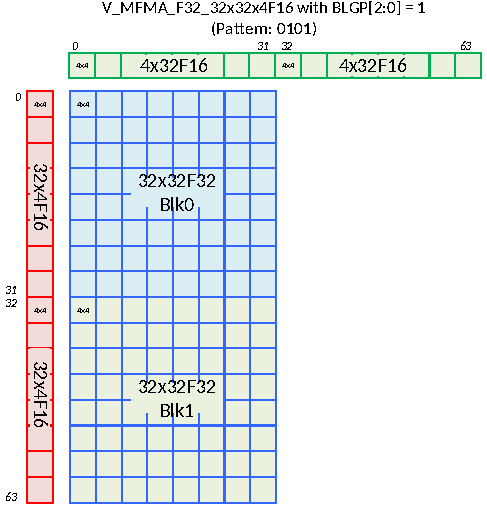
\includegraphics[width=.3\textwidth]{mfma_64x32_blgp=1}};
  %% connect the matrixA and matrixB for the mfma instruction
  \draw [->, >=stealth] ($(bufferATL)+(0, -1.5*\kBase*\unit)$) to[out=-135, in=90]
  ($(mfmaTL)+(.6, -1.15)$);
  \draw [->, >=stealth] ($(bufferBTL)+(0, -6.5*\kBase*\unit)$) to[out=-135, in=0]
  ($(mfmaTL)+(5.5, -.9)$);
  %% matrix C/D layout
  \coordinate (matrixCDTL) at ($(mfmaTL)+(7,0)$);
  \node [below right] at (matrixCDTL) {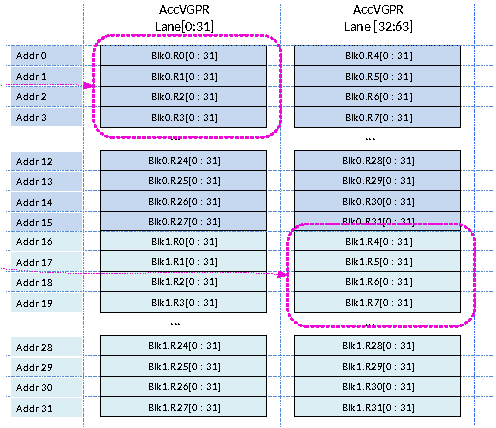
\includegraphics[width=.4\textwidth]{matrix_cd_layout}};
  %% boundary of buffer C for thread 0
  \coordinate (bufferCTL) at ($(matrixCDTL)+(1.6, -.8)$);

  \coordinate (mfmaTL2) at ($(bufferATL)+(0, -\mRepeats*\kPerBlock*\unit-\gap-6.5)$);
  \node [below right] at (mfmaTL2) {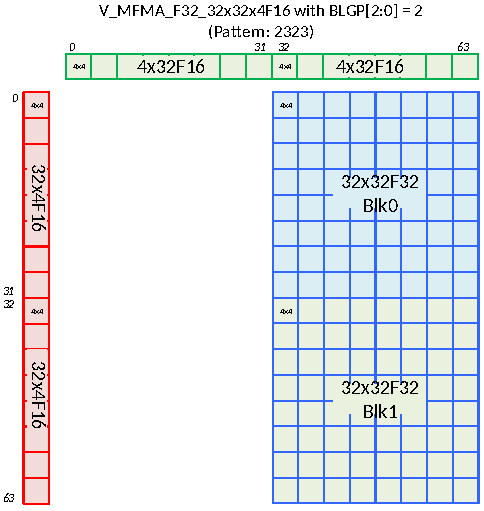
\includegraphics[width=.3\textwidth]{mfma_64x32_blgp=2}};
  %% matrix C/D layout
  \coordinate (matrixCDTL2) at ($(mfmaTL2)+(7,0)$);
  \node [below right] at (matrixCDTL2) {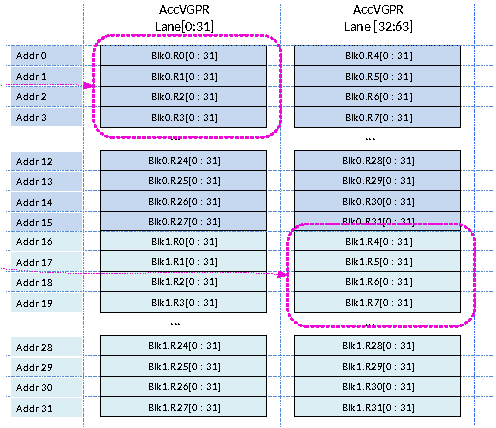
\includegraphics[width=.4\textwidth]{matrix_cd_layout}};

  \foreach \tid in {0,...,52} {
    \draw [fill opacity=.2, fill=\tileCCol, draw opacity=.2] ($(bufferCTL)+(\tid*\unit, 0)$) rectangle ++(\unit, -5.43-6.5);
    \ifthenelse{\tid=0}
    {\node [rotate=90, scale=.5, left, xshift=-.3em] at ($(bufferCTL)+(.5*\unit+\tid*\unit, -5.4-6.5)$) {workitem \tid};}{}
    \ifthenelse{\tid=52}
    {\node [rotate=90, scale=.5, left, xshift=-.3em] at ($(bufferCTL)+(.5*\unit+\tid*\unit, -5.4-6.5)$) {workitem 63};}{}
    \ifthenelse{\tid=26}
    {\node [below, yshift=-.3em] at ($(bufferCTL)+(.5*\unit+\tid*\unit, -5.4-6.5)$) {buffer C};}{}
  }

  %% xdlops1-0 and xdlops1-1
  \node at ($(mfmaTL)+(4, -3.5)$) {xdlops1-0};
  \node at ($(mfmaTL2)+(2, -3.5)$) {xdlops1-1};
}

%%% Local Variables:
%%% mode: latex
%%% TeX-master: "volkov_model"
%%% End:
